% \documentclass[journal]{vgtc}               % final (journal style)
\documentclass[review,journal]{vgtc}          % review (journal style)
%\documentclass[widereview]{vgtc}             % wide-spaced review
%\documentclass[preprint,journal]{vgtc}       % preprint (journal style)

\ifpdf%                                % if we use pdflatex
  \pdfoutput=1\relax                   % create PDFs from pdfLaTeX
  \pdfcompresslevel=9                  % PDF Compression
  \pdfoptionpdfminorversion=7          % create PDF 1.7
  \ExecuteOptions{pdftex}
  \usepackage{graphicx}                % allow us to embed graphics files
  \DeclareGraphicsExtensions{.pdf,.png,.jpg,.jpeg} % for pdflatex we expect .pdf, .png, or .jpg files
\else%                                 % else we use pure latex
  \ExecuteOptions{dvips}
  \usepackage{graphicx}                % allow us to embed graphics files
  \DeclareGraphicsExtensions{.eps}     % for pure latex we expect eps files
\fi%

%% it is recomended to use ``\autoref{sec:bla}'' instead of ``Fig.~\ref{sec:bla}''
\graphicspath{{figures/}{pictures/}{images/}{./}} % where to search for the images

\usepackage{epstopdf}
\usepackage{microtype}
\PassOptionsToPackage{warn}{textcomp}
\usepackage{textcomp}
\usepackage{mathptmx}
\usepackage{times}
\renewcommand*\ttdefault{txtt}
\usepackage{cite}
\usepackage{tabu}
\usepackage{booktabs}
\usepackage{wrapfig}
\usepackage{longfbox}
\usepackage{amssymb}
\usepackage{paralist}
\usepackage{xfrac}
\usepackage{url}
\usepackage{algorithm, algpseudocode}
\usepackage{algpseudocode}
\usepackage{amsmath}
\usepackage{framed}
\usepackage{multirow}
\usepackage{xcolor}
\usepackage{todonotes}
\usepackage[shortlabels]{enumitem}
% \usepackage[xcolor=dvipdf]{changes}
\usepackage[xcolor=dvipdf, final]{changes}
\usepackage{ulem}
\usepackage{color,soul}
\definecolor{mygreen}{rgb}{0.17, 0.55, 0.05}
\definecolor{myred}{rgb}{0.85, 0.17, 0.05}
\definecolor{text-highlight}{rgb}{0.25, 0.62, 0.29}
\sethlcolor{text-highlight}
\usepackage[T1]{fontenc} % solving problem: LaTeX Error: Command \k unavailable in encoding OT1.

\usepackage{CJKutf8} %! FOR CHINESE

\usepackage{dcolumn}
\newcolumntype{d}[1]{D{.}{.}{#1}}

\newif\ifrenderappendix
% render the appendix or not
\renderappendixfalse
% \renderappendixtrue

\definechangesauthor[name=JiachengPan, color=mygreen]{pan}
\definechangesauthor[name=XiaodongZhao, color=red]{zhao}
\definechangesauthor[name=Jian Chen, color=blue]{jc}
\setdeletedmarkup{\color{gray}{\sout{#1}}}
% \setdeletedmarkup{}
% \sethighlightmarkup{\color{red}{#1}}
\setaddedmarkup{\color{mygreen}{#1}}
\setauthormarkup{}
\renewcommand{\algorithmicrequire}{\textbf{Input:}}
\renewcommand{\algorithmicensure}{\textbf{Output:}}

\definecolor{lightgray}{rgb}{0.75,0.75,0.75}
 
\newenvironment{lightgrayleftbar}{%
  \def\FrameCommand{\textcolor{lightgray}{\vrule width 3pt} \hspace{3pt}}%
  \MakeFramed {\advance\hsize-\width \FrameRestore}}%
{\endMakeFramed}

\newcommand{\ApproachName}{GraphAugmentor}
\newcommand{\PaperTitle}{\ApproachName: Augmenting Node-Link Diagrams With Textual Descriptions} % todo


\onlineid{1396}

\vgtccategory{Research} % TODO
\vgtcpapertype{Representations \& Interaction} % TODO

\title{\PaperTitle}
\author{Jiacheng Pan, Zihan Yan, Zihan Zhou, Xiaodong Zhao, Shenghui Cheng, Dongming Han, Jian Chen, Mingliang Xu, Wei Chen}
\authorfooter{
    % \item Jiacheng Pan, Zihan Yan, Zihan Zhou, Xiaodong Zhao, Dongming Han, and Wei Chen are with the State Key Lab of CAD\&CG, Zhejiang University, China. E-mail: \{panjiacheng, zhouzihan,  zhaoxiaodong\}@zju.edu.cn, chenwei@cad.zju.edu.cn.\\
    % Wei Chen is the corresponding author.
    
    % \item Jian Chen is with Ohio State University, USA. E-mail: chen.8028@osu.edu.
}

\shortauthortitle{Pan \MakeLowercase{\textit{et al.}}: \PaperTitle}
    \abstract{
    Node-link diagrams are the most popular form for graph visualization.
    Yet, salient information and visual structures of a graph can not be fully depicted by solely presenting its node-link diagram.
    We propose to augment the comprehensibility of node-link diagrams by creating textual descriptions. 
    We conduct a pilot study to identify eight requirements of generated interpretations, including four items for connection extraction and four items for visual expression.
    Our solution, \textit{\ApproachName}, generating interactive descriptions for the widely-used Scalable Vector Graphics (SVG) format node-link diagrams, consists of two stages: feature extraction and description generation. 
    The first one identifies and extracts visual features, like node-link connections, visual designs, and types of graph layouts.
    The second stage creates a group of hierarchical sentences based on a pre-defined schema. 
    To the best of our knowledge, our approach is the first attempt to textually convey the visual design of node-link diagrams automatically. 
    Three use cases and in-lab user study confirm the superiority of our approach.
    }
    
    \keywords{Node-link diagram, graph visualization, visual encodings, visual representations}

%% ACM Computing Classification System (CCS). 
%% See <http://www.acm.org/class/1998/> for details.
%% The ``\CCScat'' command takes four arguments.

\CCScatlist{ % not used in journal version
 \CCScat{K.6.1}{Management of Computing and Information Systems}%
{Project and People Management}{Life Cycle};
 \CCScat{K.7.m}{The Computing Profession}{Miscellaneous}{Ethics}
}

\ifrenderappendix
    \teaser{}
\else
    \teaser{
      \centering
      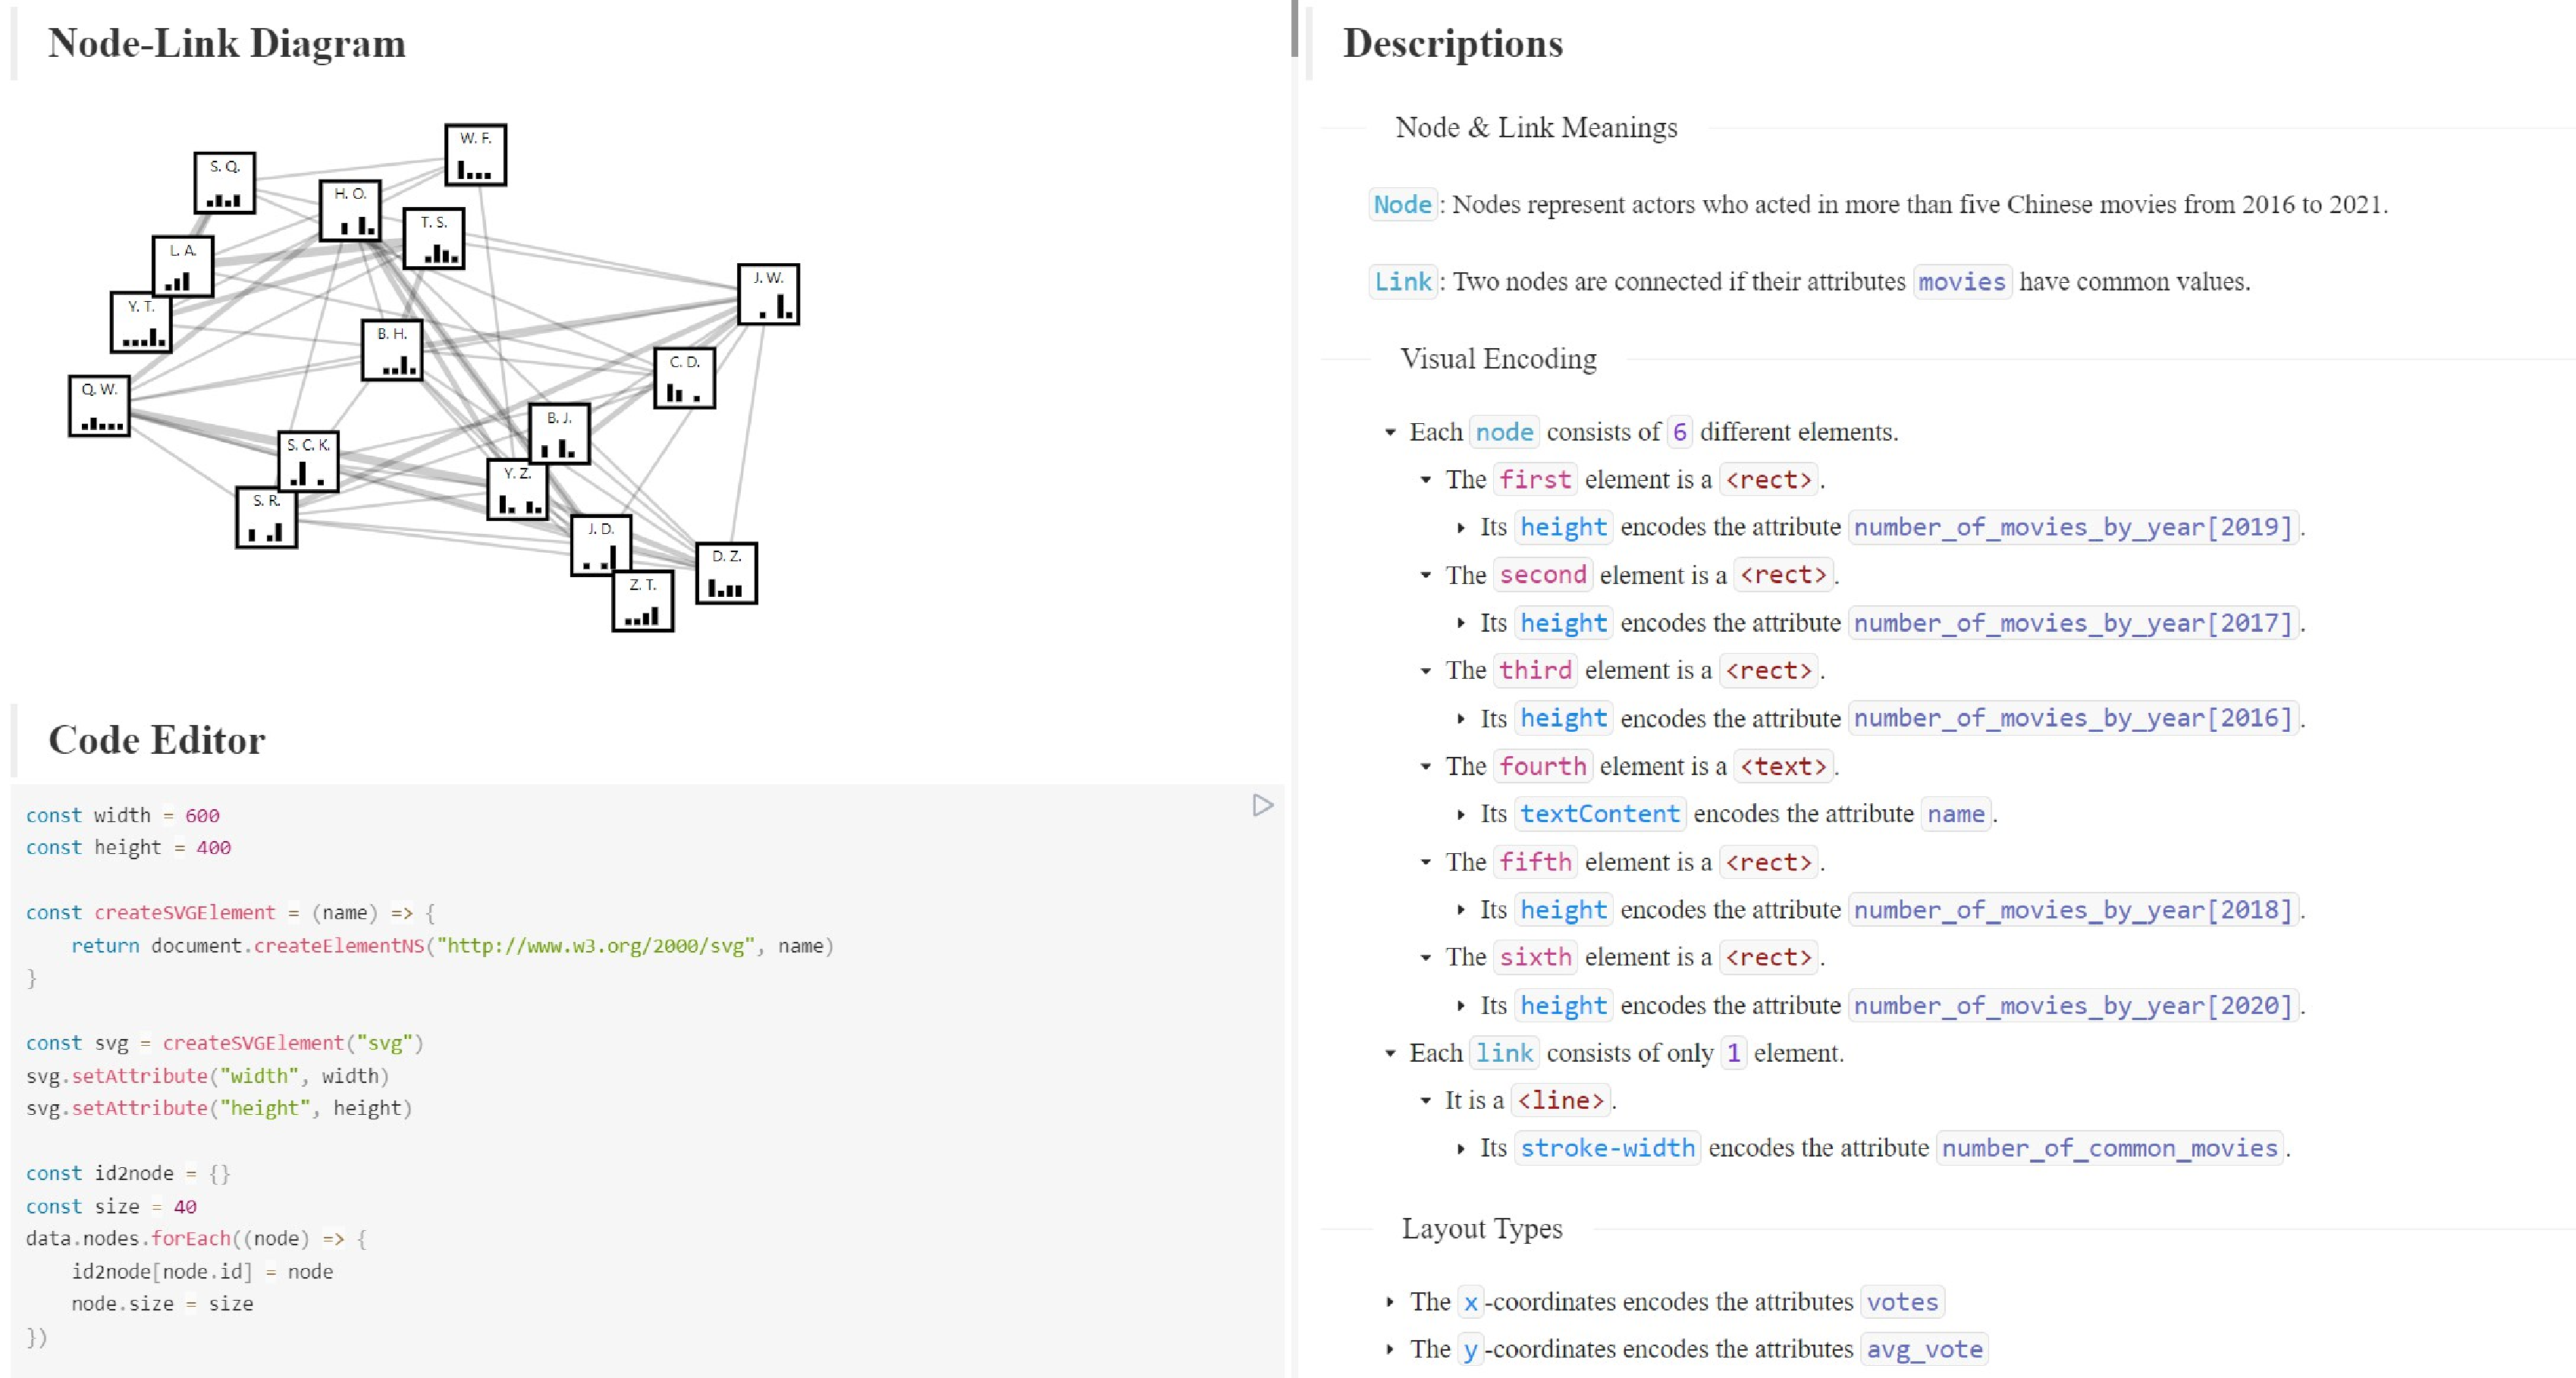
\includegraphics[width=1\linewidth]{figures/teaser.eps}
        \caption{
            The pipeline of~\ApproachName.
            (a) The node-link diagram created with the Actor-China graph (17 nodes and 25 links). (b) The feature extraction modules summarize link conditions, visual encodings, and the layout type of the diagram. (c) The generator interprets the summarized features with interactive descriptions. (d) The generated descriptions are interactive. Hovering on descriptions will highlight their corresponding visual elements (e).
            % The interface of~\ApproachName.
            % (a) The node-link diagram created upon the Actor-Movie-2016-2021-China Dataset.
            % The graph consists of 17 nodes (actors in china who have acted in more than five movies from 2016 to 2021) and 55 links (two actors are connected if they acted in at least one movie). (b)~\ApproachName~generates descriptions to explain the graph automatically, including the meanings of nodes and links, visual encodings, and the layout meanings. Descriptions are linked to the visualization to make them more targeted. (c) Hovering on a certain description will toggle highlighting on the visual element it describes.
        }
        \label{fig:teaser}
    }
\fi

\vgtcinsertpkg
\begin{document}
\begin{CJK}{UTF8}{gbsn} %! FOR CHINESE

\ifrenderappendix
    \maketitle
\section{Node-Link Diagrams in the User Interview}

\begin{table}
\centering
\caption{\label{tab:pearson-correlation}The Pearson correlation coefficients testing correlations between Euclidean distances and graph geodesic distance with 15 graphs and 5 different layouts. Cells with coefficients less than $\theta=0.5$ are highlighted. $p$-values are all zero.}
\label{tab:pearson-correlation}
\begin{tabular}{llllll} 
\hline
Dataset       & FM$^3$ & F.R.           & S.M.  & PMDS  & R.T.            \\ 
\hline
dwt\_72       & 0.894  & 0.552          & 0.94  & 0.897 & 0.714           \\
lesmis        & 0.804  & 0.728          & 0.815 & 0.779 & 0.504           \\
bcsstk09      & 0.967  & 0.610          & 0.971 & 0.947 & 0.754           \\
cage8         & 0.658  & 0.678          & 0.725 & 0.701 & \textbf{0.307}  \\
can\_96       & 0.835  & 0.824          & 0.855 & 0.869 & \textbf{0.426}  \\
dwt\_1005     & 0.969  & 0.561          & 0.974 & 0.972 & 0.623           \\
dwt\_419      & 0.979  & \textbf{0.391} & 0.987 & 0.987 & 0.775           \\
grid17        & 0.968  & 0.551          & 0.976 & 0.964 & 0.738           \\
jazz          & 0.826  & 0.821          & 0.813 & 0.786 & \textbf{0.297}  \\
mesh3e1       & 0.99   & 0.502          & 0.996 & 0.995 & \textbf{0.465}  \\
netscience    & 0.901  & 0.573          & 0.93  & 0.919 & 0.752           \\
price\_1000   & 0.783  & \textbf{0.376} & 0.808 & 0.786 & 0.727           \\
rajat11       & 0.753  & 0.670          & 0.868 & 0.847 & 0.618           \\
soc-wiki-Vote & 0.798  & 0.775          & 0.821 & 0.757 & \textbf{0.316}  \\
visbrazil     & 0.937  & 0.828          & 0.941 & 0.958 & 0.758           \\
\hline
\end{tabular}
\end{table}
\else
    \firstsection{Introduction}
\maketitle
% 修改想法:从reverse-engineering的角度出发来重新讲整个故事会更容易。
% ! [1][background and problem] The wide-using of node-link diagrams, 很多创作者使用svg来创作节点链接图,但如果节点链接图的创作者仅仅向受众传达节点链接图本身,而不交代编码信息,无法向受众良好的传达想要表达的意义;
% ! [2][motivation] 创作者可以添加一些附加的components,比如legends、文本描述 或者 tooltips 来辅助受众理解他创作的节点链接图。其中最关键的步骤则是收集创作者创建节点链接图用到的编码方案。虽然创作者对于他创作的节点链接图心知肚明,但仍需要将他所用到的编码重新手动汇总,以进一步使用这些信息来生成附加组件。我们的方法想要减少创作者手动汇总编码信息的劳动,并且提供了一些能够帮助用户理解可视化编码的附加组件,创作者也可以利用提取到的编码信息来生成自定义的附加组件。自动提取编码信息,还能重新审视自己的可视化算法是否存在编码错误的bug。
% ! [3][challenges] 根据xxx等人的调研[x, x, x],很多工作将节点和链接上的属性分别编码在它们对应的可视化图形上。提取这些编码依赖于检查可视化图形和节点、链接的对应关系,以及图形通道和节点、链接的对应关系。因为节点链接图存在很多视觉遮挡,直接作用于pixel picture的工具很难提取其中包含的编码。而应用在svg上的工具,比如xx,则依赖于作者将数据源绑定在graphics上,并且其无法区分节点和链接,难以应用在节点链接图上。因为我们的方法服务于可视化创作者,他可以直接在开发可视化的过程中使用我们的工具,从而我们聚焦于从可视化算法中提取编码信息,这也使得编码的提取成为可能,因为可视化算法中包含了编码信息。





Node-link diagrams are widely used to depict relations among data entities and associated attributes. 
% These attributes are mapped to visual channels (e.g., the shape, size, and color of a node encode three different attributes in Figure~\ref{fig:BasicCases} (b)) to reveal attribute-based patterns. 
Various visual channels (e.g., position, shape, size, and color) are employed to encode attributes.
However, excessive number of attributes will lead to a heavy cognitive load 
% for human observers to interpret and visually extract 
to perceive information and identify patterns effectively, which brings more impact on novice users with low visualization literacy.
%It is also often that a non-professional user has a low ability of reading visual forms, especially when there are a large amount of visual elements. 
Our idea in this work is to automatically generate descriptions for a multi-attribute node-link 
diagram to enhance the mental understandings to the underlying diagram. 
% diagrams from the perspective of demonstrating the creating process of a node-link diagram, which facilitates humans' comprehension for the rich information in the diagram.


Generating a summarized description for 
% a visualization facilitates its audience to understand its underlying meaning. 
a statistical chart has been popular for its capability of characterizing the meaning of the visualization. 
Existing works 
% for automatic description generation 
classes 
can be categorized into two areas~\cite{DBLP:conf/inlg/ObeidH20}: one describes constituents and visual encodings of a  visualization~\cite{DBLP:journals/coling/MittalMCR98, DBLP:journals/tochi/FerresLST13}, and the other describes high-level insights conveyed by the visualization~\cite{DBLP:conf/apvis/LiuXHWY20, DBLP:conf/inlg/ObeidH20}. By analogizing with the taxonomy of visualization annotation techniques~\cite{DBLP:conf/chi/HullmanDA13}, descriptions generated by 
% the above two 
both 
categories 
% of techniques 
can also be referred to \textit{observational descriptions} and \textit{additive descriptions}. 
% However, techniques for automatically generating descriptions for node-link diagrams have not been explored yet due to the limitations of the above techniques.
However, these approaches are not applicable for node-link diagrams:

\textbf{Observational techniques} assume that constituents (e.g., axes, bars, and legends) of basic charts are well-defined. 
For example, 
% Mittal et al.~\cite{DBLP:journals/coling/MittalMCR98} require 
pre-defined visual mapping relationships 
are demanded~\cite{DBLP:journals/coling/MittalMCR98} 
to generate captions.
In other approaches, textual information of axes and legends is needed~\cite{DBLP:conf/icip/ZhouT00, DBLP:conf/doceng/HuangT07, DBLP:conf/grec/HuangTL03}.
% and other techniques rely on the textual information of axes and legends~\cite{DBLP:conf/icip/ZhouT00, DBLP:conf/doceng/HuangT07, DBLP:conf/grec/HuangTL03}.
% However, textual information in dense node-link diagrams is always hidden to avoid visual clutter. 
This scheme can not be used for dense node-link diagrams since the textual annotations of the nodes and edges need to be hidden to avoid visual clutter.
% Additionally, the complexity of analytical tasks has put forward the challenge of creating more informative diagrams (often achieved by integrating complex glyphs into a node-link diagram to encode the associated attributes), e.g., nesting basic charts into nodes~\cite{gehlenborg2010visualization, DBLP:conf/iv/JusufiDK10} and customizing shapes of links~\cite{DBLP:conf/iv/SchoffelSE16, DBLP:journals/tvcg/NielsenJBJ09}. This further increases the difficulty of interpreting a node-link diagram.
In addition, customized visual encodings in node-link diagrams, such as nesting basic charts into nodes~\cite{gehlenborg2010visualization, DBLP:conf/iv/JusufiDK10} and utilizing alternative shapes for links~\cite{DBLP:conf/iv/SchoffelSE16, DBLP:journals/tvcg/NielsenJBJ09}, make the description of multi-attribute node-link diagrams more challenging. 

\textbf{Additive techniques} generate descriptions from the underlying tabular data based on pre-defined or restricted insights~\cite{DBLP:journals/pvldb/DemiralpHPP17, DBLP:journals/tvcg/WangSZCXMZ20, DBLP:conf/apvis/LiuXHWY20, DBLP:conf/chi/KimHA20}. However, insights in a node-link diagram depend on the topological structure 
% and
, and thus
can be more flexible.


In this paper, we make the very first attempt to generate observational descriptions of node-link diagrams.
% (the first category) considering the remaining technical difficulties for additive descriptions (the second category). 
We contribute~\textit{\ApproachName}, an automatic description generator for node-link diagrams in the format of Scalable Vector Graphics (SVG). 
It extracts key information of a diagram from the underlying graph and the source code by following the creating process of node-link diagrams~\cite{DBLP:journals/cgf/SpritzerBDFF15, tvcg/RomatAP21}:
\textbf{1) graph wrangling} transforms the original tabular data into a graph format by defining relationships (links) between entities (nodes);
\textbf{2) visual encoding} maps node/link attributes to visual channels;
\textbf{3) layout computing} positions nodes in a two-dimensional space to reveal attribute-based or topology-based patterns~\cite{DBLP:journals/cgf/NobreMSL19}.
Particularly, \ApproachName~
% first checks the links between all nodes, and 
selects potential links to interpret the \textbf{graph wrangling} process.
Then it obtains \textbf{visual encodings} by continuous data modifications and identifying their effects on the visualization result.
% Ultimately, 
\ApproachName~interprets the \textbf{layout computing} step by examining the factors that influence node positions.
% The extracted information is fed into pre-defined templates to generate textual descriptions. Particularly, we implement an interface to display textual descriptions and support interactive highlight of the text contents by hovering on the corresponding area of the diagram.
A pre-defined template is used to create textual descriptions based on extracted information. 
We design and implement a visual interface to support interactive specification, exploration and modulation of descriptions.
The usability and effectiveness of \ApproachName~are demonstrated by four case studies and a user study.
The contributions of this paper are twofold:

\noindent \textbf{1)} An automatic description generation approach interprets the creating process of a node-link diagram by template-based descriptions.

\noindent \textbf{2)} A visual encoding extraction method retrieves visual encoding schemes from the underlying graph and the code creating diagrams.
    \section{Related Work}\label{sec:relatedwork}
%! related work 的目的,是给审稿人看你的文章到底做了什么,到底哪些工作是跟你类似的,需要在这里跟他们撇清关系。
\subsection{Attributed Node-link Diagram}
Node-link diagrams are widely used to reveal topology and relationships between entities.
We aim to generate descriptions for node-link diagrams with visual encodings.
Nobre et al.~\cite{DBLP:journals/cgf/NobreMSL19} surveyed numerous multivariate graph visualization techniques,
and Partl et al.~\cite{DBLP:conf/biovis/PartlKLKSS12} discussed four categories of attributed node-link diagram layouts.
Node-link diagrams can encode attributes of nodes and links by visual elements.

% 对节点而言,最基础的编码可以将标签编码为文本,将节点的大小编码数值型属性,将节点的颜色编码类别型属性。
% 更复杂的编码中,节点还被编码成一个嵌入的图表,
Node attributes are basically encoded by their size, color, and shape.
Techniques encoding diverse attributes usually nest complex constitutions into one node~\cite{DBLP:conf/infovis/AuberCJM03}.
For example, nodes can be visualized as line charts, box plots, and bar charts in the biology domain~\cite{gehlenborg2010visualization, DBLP:conf/iv/JusufiDK10}.
Photos, icons, or customized glyphs are also often used to encode node attributes~\cite{DBLP:conf/chi/DunneS13}.
Graph visualization tools such as Cytoscape~\cite{DBLP:journals/bioinformatics/FranzLHDSB16}, Gephi~\cite{DBLP:conf/icwsm/BastianHJ09}, NetV.js~\cite{HAN2021} can handle varying degrees of attribute-embedding in node-link diagrams.
The layout is also a crucial element of node-link diagrams.
Node positions are computed by topology-driven layout algorithms~\cite{DBLP:journals/spe/FruchtermanR91, DBLP:journals/cgf/KruigerRMKKT17, DBLP:journals/tvcg/GansnerHN13, DBLP:journals/tvcg/ZhuCHHLZ21} to reveal topology structures.
But attribute-driven layouts are preferred in several cases.
For example, spatial graphs contain geographic coordinates and the position of a node can encode the longitude and latitude~\cite{DBLP:journals/tvcg/ElzenW14, DBLP:journals/tvcg/Guo09}.

Visual channels of links such as width~\cite{Katz_2015}, color~\cite{DBLP:journals/tvcg/Guo09}, and dashes~\cite{DBLP:journals/bmcbi/JunkerKS06} can also support attributed links,
although links have less space for attribute encoding that nodes.
In more complex cases, links can incorporate multiple visual elements.
Sch{\"{o}}ffel et al.~\cite{DBLP:conf/iv/SchoffelSE16} encoded the link with bar charts to visualize multiple link attributes.
Abyss Explorer~\cite{DBLP:journals/tvcg/NielsenJBJ09} ``wiggles'' the links and encode attributes of a link with its length.
% Compared to nodes, links have less space for attributes encoding.
% 这些工作为我们的工作提供了很多很优秀的案例,我们的工作将会围绕这些案例进行展开,为带有不同编码方案的节点链接图生成相关描述作为标题。
These techniques provide numerous cases for our approach. 
We aim to generate relevant descriptions for node-link diagrams with various encoding schemes.

\subsection{Information Extraction of Visualization}
% ! Data
Numerous methods interpret visualizations by retrieving data from raster images.
Usually, methods that deal with multiple types provide algorithms to classify charts in the beginning~\cite{DBLP:conf/icip/GaoZB12, DBLP:conf/chi/JungKSHLKS17, DBLP:conf/eccv/SiegelHLDF16, DBLP:journals/vlc/DaiWNZ18}.
These methods often employ Optical Character Recognition (OCR) to extract textual information from captions, labels, and axes~\cite{DBLP:conf/icip/ZhouT00, DBLP:conf/doceng/HuangT07, DBLP:conf/grec/HuangTL03}.
The combination of OCR and graphics detection techniques facilitates data retrieval in these methods.
Other kinds of charts~\cite{DBLP:conf/pkdd/ClicheRMY17, DBLP:conf/uist/SavvaKCFAH11} are handled by extending these methods to more diverse tasks.
iVolVER~\cite{DBLP:conf/chi/MendezNV16} supports transformation of the extracted data to construct interactive animated visualizations.
ReVision~\cite{DBLP:conf/uist/SavvaKCFAH11} populates a gallery of alternative redesigned visualizations through data extraction.
More recently, Chartem~\cite{DBLP:journals/tvcg/FuZCGWZHTZM21} extracts data and embeds it back into the chart to facilitate visualization spread.
More related to graphs, Henkel et al.~\cite{DBLP:conf/vmv/HenkelKLG20} and Lee et al.~\cite{DBLP:conf/icdar/LeeYWH17} retrieved tree-structured data from treemaps and dendrograms.
Several other approaches have been proposed to assist those with impaired vision~\cite{DBLP:conf/ismis/ChesterE05, DBLP:journals/tiis/CarberrySMDWGCSOM12, DBLP:journals/cgf/ChoiJPCE19}.


% ! Insights
Another type of method extracts insights from visualizations~\cite{DBLP:conf/diagrams/WuCEC10, DBLP:journals/nrhm/DemirOSECMC10} and their underlying data~\cite{DBLP:conf/inlg/ObeidH20, DBLP:journals/ivs/CuiBYE19}.
Demiralp et al.~\cite{DBLP:journals/pvldb/DemiralpHPP17} defined \textit{insights} as strong manifestations of the data or the visualization.
Different methods have different preferences according to their inputs.
For example, inputs of Chart-to-Text~\cite{DBLP:conf/inlg/ObeidH20} mainly come from the underlying data.
In contrast, Wu et al.~\cite{DBLP:conf/diagrams/WuCEC10} and Demir et al.~\cite{DBLP:journals/nrhm/DemirOSECMC10} employed visual features,
and identified the intention of line charts and bar charts by detecting the most significant features.
AutoCaption~\cite{DBLP:conf/apvis/LiuXHWY20} first parses textual and visual components to a formatted information table incorporating the underlying data,
then extracts a set of predefined features as insights from the table.
Several systems employ the extracted insights to augment visualizations by annotation~\cite{DBLP:conf/ieeevast/Kandogan12, DBLP:journals/tvcg/BryanMW17}, overlays~\cite{DBLP:journals/tvcg/KongA12},  and widgets~\cite{DBLP:journals/tvcg/SrinivasanDES19}.
% Kandongan~\cite{DBLP:conf/ieeevast/Kandogan12} introduced the concept of just-in-time descriptive analytics to help users understand data in point-based visualizations (e.g., scatter plots, line charts, et cetera). 
% The fundamental is to identify clusters, outliers, and trends from visualizations.
% Srinivasan et al. presented Voder~\cite{DBLP:journals/tvcg/SrinivasanDES19}, a system to generate data facts (descriptions of data statistics) based on a basic set of heuristics.
% Then the facts are used as interactive widgets to improve user interpretion.
% Graphical Overlays~\cite{DBLP:journals/tvcg/KongA12} takes the insights to generate graphical overlays on charts to draw the viewer's attention.

These two categories of methods retrieve the underlying data from visualization results and generate insights from the extracted information. 
They mainly focus on classical charts such as line charts, bar charts, and pie charts.
We concern more about the constituents of a node-link diagram, such as its visual encodings and layout.

%! visual mapping
Poco and Heer~\cite{DBLP:journals/cgf/PocoH17} proposed a reverse-engineering approach to recover visual encodings from area charts, bar charts, line charts, and scatter plots (though they did not infer such visual channels as color, shape, and size).
Then they made up for the lack of color mapping by using OCR techniques to detect continuous legends~\cite{DBLP:journals/tvcg/PocoMH18} and discrete legends~\cite{DBLP:conf/sibgrapi/MayhuaNHP18}.
Yuan et al.~\cite{DBLP:journals/corr/abs-2103-00741} presented a deep learning method to detect the color mappings without textual legends.
These methods mainly extract visual encodings from raster images, but with the emergence of D3~\cite{DBLP:journals/tvcg/BostockOH11}, web-based visualization is more popular now.
Visual encoding extraction can be more diverse and accurate with D3's the data-binding feature.
Harper and Agrawala~\cite{DBLP:conf/uist/HarperA14} introduced a tool to deconstruct D3 visualizations by extracting the bound data, markers, and visual mappings. 
They enhanced the tool to use identified textual information to generate reusable style templates~\cite{DBLP:journals/tvcg/HarperA18, DBLP:journals/tvcg/HoqueA20}. % enhanced the tool again with more detection target such as angles, arcs, and so on. With the tool, they presented a search engine that can index D3 visualizations based on the extarcted information.

% 这些方法或是只适用于检测基础的可视化图表如bar chart/line chart/area chart等,或是只适用于对d3等具有数据绑定的svg进行编码提取。
% 我们提出了对节点链接图进行信息提取的方法,该方法从多个角度出发,适用于通用的svg场景,而不需要数据绑定的前提。
Methods that extract visual mappings from raster images~\cite{DBLP:journals/cgf/PocoH17, DBLP:journals/tvcg/PocoMH18, DBLP:conf/sibgrapi/MayhuaNHP18, DBLP:journals/corr/abs-2103-00741} can be more applicable to common cases, but they are primarily designed for basic charts or only can detect only predefined visual mapping types.
Methods that deconstruct D3 visualizations~\cite{DBLP:conf/uist/HarperA14, DBLP:journals/tvcg/HarperA18, DBLP:journals/tvcg/HoqueA20} can be applied to more kinds of visual mappings, but they require D3's data-binding feature so that data can be retrieved for visual elements. The method proposed here supports extracting visual encodings for SVG formatted node-link diagrams without data bound to visual elements.

\subsection{Automatic Description for Visualization}
Approaches that generate descriptions for visualizations are mainly based on the extracted information.
Mittal et al.~\cite{DBLP:journals/coling/MittalMCR98} developed a caption-generation system with natural language-generation techniques to describe mappings between data and marks.
Similarly, iGraph-Lite~\cite{DBLP:journals/tochi/FerresLST13} generates template-based descriptions of the appearance of a chart.
Other approaches stress generating descriptions of extracted insights.
Chart-to-Text~\cite{DBLP:conf/inlg/ObeidH20} generates natural language descriptions for line charts and bar charts using the transformer model~\cite{DBLP:conf/nips/VaswaniSPUJGKP17}. 
Similarly, AutoCaption~\cite{DBLP:conf/apvis/LiuXHWY20} puts the extracted insights into templates to generate captions about trends, maximum values, clusters, and the like.
% 一些工作通过回答问题的方式来提取insight.
Several approaches generate descriptions by answering questions about visualizations.~\cite{DBLP:conf/cvpr/KaflePCK18, DBLP:conf/chi/KimHA20, DBLP:conf/eccv/KembhaviSKSHF16}.
Kembhavi et al.~\cite{DBLP:conf/eccv/KembhaviSKSHF16} interpret the relationships among multiple scientific diagrams in one picture;
a dataset called DVQA~\cite{DBLP:conf/cvpr/KaflePCK18} is given with more than 3 million image-question pairs about bar charts to support bar chart question answering. 
An end-to-end neural network and a dynamic local dictionary are designed to indicate the ability of the dataset.
More recently, Kim et al.~\cite{DBLP:conf/chi/KimHA20} introduced an automatic question answering pipeline to answering natural language questions about bar charts and line charts; this system extends Sempre~\cite{DBLP:conf/acl/PasupatL15, DBLP:conf/emnlp/ZhangPL17} to answer questions about charts with Vega-Lite~\cite{DBLP:journals/tvcg/SatyanarayanMWH17} format and give visual explanations.

% None of these approaches is tailored for generating descriptions for node-link diagrams. 
% We propose an approach named \ApproachName~to generate descriptions for node-link diagrams automatically.
% It utilizes three information extraction pipelines to detect crucial information from the source code and the underlying graph and generates template-based descriptions.
    \section{Requirement and Overview}\label{sec:pilotstudy}

As surveyed in Section~\ref{sec:relatedwork}, there are two main steps to augment the node-link diagram: information extraction and description. Thus, we conducted a pilot study aiming to investigate the requirements for these two steps from the viewpoints of both 3 experts (P1-3) and 12 end-users (P4-15). We showed them some typical and various sample node-like diagrams with legends. Based on their relevant feedback, we analyzed the approach requirement and proposed an overview of our approach.

\subsection{Requirement Analysis}

Based on our analysis, we came up with four requirements [E1-4] for information extraction and three requirements [D1-3] for description generation.

\noindent {\bf Extracting Information.}

\begin{compactenum}[\textbf{E}1]
    \item {\bf Searching link condition.} The meanings of links should be demonstrated directly to end-users. Unlike nodes, users cannot find the meaning of a link on the title or caption of a graph. Hence, all experts suggested we summarize the meanings of links for users before they carefully analyze the graph. Experts also gave more refined suggestions pertaining to our approach of finding the correct link condition~\cite{DBLP:journals/ivs/LiuNS14, DBLP:journals/ivs/HeerP14, DBLP:journals/tvcg/SrinivasanPEB18} among nodes to help users understand the meaning of links automatically.
    
    \item {\bf Summarizing visual encodings.} Visual encoding is a necessary part for users to understand the graph. Although legends always represent it, they are too concise for users to understand. Furthermore, both P4 and P7 commented that despite their ability to comprehend visual encodings, it was wasteful to search attributes for each node and link according to their visual elements and legends. Thus, it is highly recommended to summarize all visual encodings, which can be demonstrated directly to users later.
    
    \item {\bf Identifing the layout type.} All experts agreed that the layout could help users understand the node-link diagram. Whereas, due to the lack of prior knowledge, most end-users ignored the layout. Experts recommended that we present only the essential information and type of layout rather than explain the algorithm details in detail to reduce end-users' understanding load. Expert P2  suggested only identifying whether the layout is topology-driven or attribute-driven, or neither, according to the taxonomy~\cite{DBLP:journals/cgf/NobreMSL19}. 
    
    \item {\bf Utilizing multi-source inputs}. Experts suggested our approach should utilize multi-source inputs, especially the original data and the visualization program. Expert P1 emphasized the importance of visualization programs, since they contain more information, such as how data attributes are encoded by visual channels, than raw data. Enriching the types of our inputs can improve the accuracy and the comprehensiveness of the collected information to avoid misleading users.
\end{compactenum}

\noindent {\bf Describing information. }
\begin{compactenum}[\textbf{D}1]
    \item {\bf Describing information with textual descriptions.} Most end-users prefer our method as it can use more detailed hints such as textual descriptions to provide more comprehensive illustrations. 
    % They mentioned that the common used legend is troublesome, first, they need to learn the mapping relationship, second, they should interpret each visual element one by one by searching the corresponding information provided by the legend. 
    Expert P2 suggested to use textual descriptions, which are more flexible to carry different content.
    The use of textual descriptions can reduce the learning cost, as well as help users focus more on analysis rather than information searching~\cite{DBLP:journals/tochi/FerresLST13, DBLP:conf/inlg/ObeidH20, DBLP:conf/apvis/LiuXHWY20}. 
    % The end-user P4 said that ``Language is the bridge of communication, and language descriptions of visualizations can bridge me to their authors.'' 
    
    \item {\bf Using templates to generate consistent descriptions.} One expert suggested that a template-based scheme is more suitable for our description generation, because it is stable and consistent to display structured descriptions in our scenario. He also suggested highlighting non-template information in the template to facilitate users' recognition.
    % End-users also prefer using template. They deemed that in tasks, they often need to find one attributes for multiple nodes. If the attributes showed on different place of descriptions, it is difficult for them to search the information and analyze.
    
    \item {\bf Organizing descriptions according to their relationship.} Because there may be several different types of information, expert P2 suggested organizing the corresponding descriptions according to their relationships. Specifically, he said that all descriptions of visual encodings of the same data entity should be displayed together without adding any additional descriptions, such as the meanings of links. It was agreed upon by all end-users that descriptions should be arranged according to the relationship as most daily document tools did, such as ``X-mind'', ``Google Doc'', ``Typora''and so on.
    
    \item {\bf Constructing mapping between graph and descriptions.} Building a linkage between our hints and the visualization can help users quickly locate and search for the target. Some end-users mentioned that the static hints (e.g., legend) obstructed their information tracking. They suggested providing an interactive mapping tool; for example, the relevant visual elements can be highlighted while hovering on their descriptions. The interactive mapping tool can make the hints more targeted and reduce mismatches with the end-users’ mental map.
\end{compactenum}

\subsection{\ApproachName~Overview} \label{sec:overview}

\begin{figure*}[t]
    \centering
    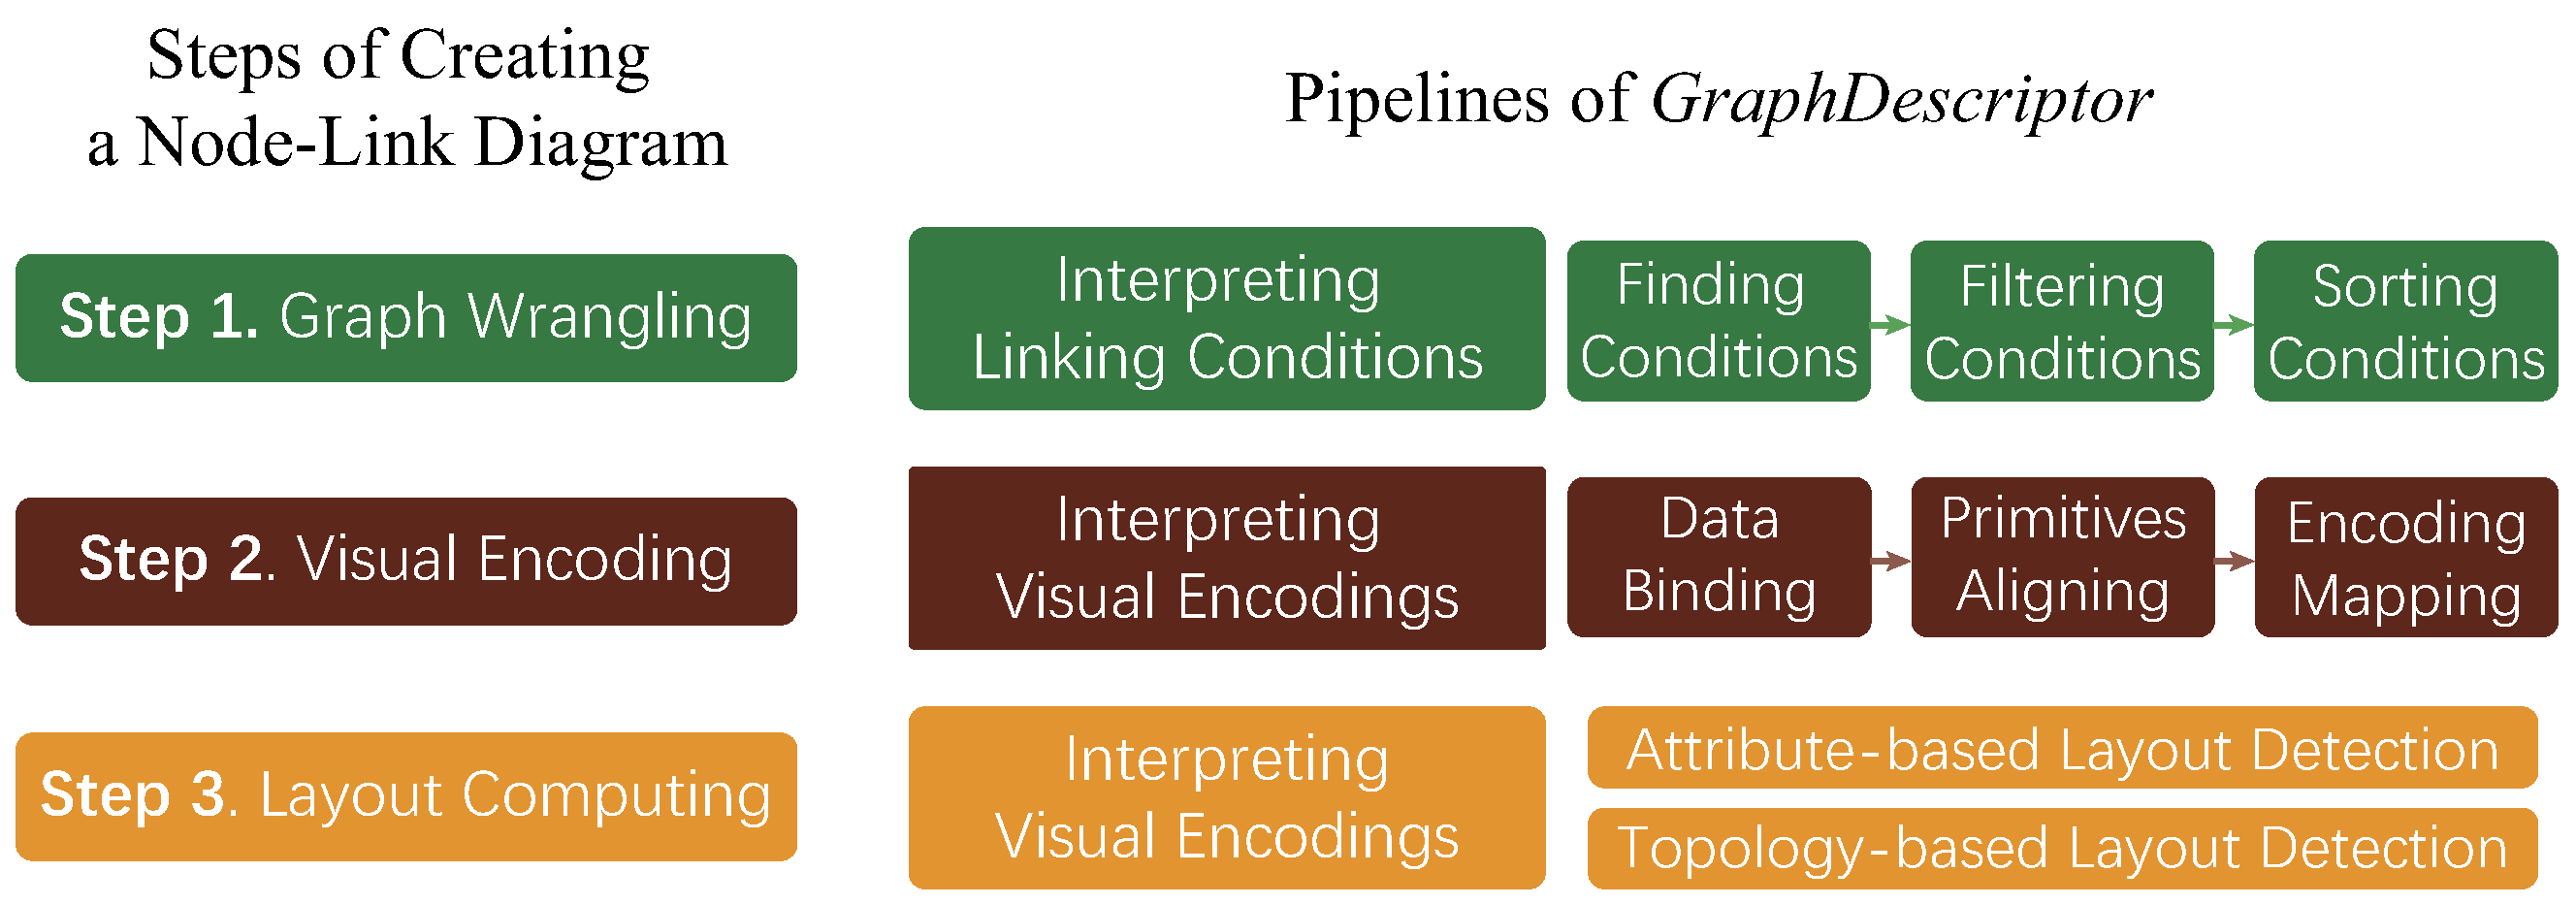
\includegraphics[width=2\columnwidth]{figures/workflow.eps}
    \caption{The pipeline of~\ApproachName. (a) Three information extraction modules search link conditions, summarize visual encodings, and identify layout types. (b) A description generator generates template-based descriptions with interactions. 
    }
    \label{fig:workflow}
\end{figure*}

Following the aforementioned requirements, we propose~\ApproachName~(Figure~\ref{fig:workflow}), an automatic description generation approach to augment the comprehensibility of node-link diagrams, which consists of three information extraction modules and an interactive description generator. They work together to extract information from node-link diagrams and generate corresponding descriptions for end-users.

\noindent {\bf Information Extraction Modules}  (Section~\ref{sec:approach}). To complete \textbf{E1-4}, we designed and implemented three information extraction modules (Figure~\ref{fig:workflow}a) with multi-source inputs (\textbf{E}) including the captured visualization programs and the original graph data.

\begin{compactenum}[\textbf{M}1]
    \item {\bf Link Condition Search Module.}
    To implement \textbf{E1}, we searched the link conditions. The module takes the original graph data as input and selects proper conditions between connected node pairs to represent the link meanings.
    
    \item {\bf Visual Encodings Summarization Module.}
    Following \textbf{E2}, our module forms the encoding scheme by summarizing mappings between data entities and visual elements and the correlations between data attributes and visual channels. It takes visualization programs and the original graph data as inputs and tests the relationship between the graph data and output visualizations to infer visual encodings.
    
    \item {\bf Layout Type Identification Module.} Based on \textbf{E3}, we proposed this module to determine whether the layout is attribute-based or topology-based. This module will capture the position of each node by computing bounding boxes, and determine the layout type by testing the Pearson correlation coefficient.
\end{compactenum}

\noindent {\bf Description Generator} (Section~\ref{sec:generator}).
According to \textbf{D1-4}, we propose a description generator
(Figure~\ref{fig:workflow}b) to express the extracted information. 
The description generation follows a manner of template-filling (\textbf{D1-2}). Although the template resembles the skeleton of the description, the spirit of the description is derived from the extracted information.
To demonstrate the relationship of different levels of descriptions (\textbf{D3}), we organized the generated descriptions in a pre-set structure. Besides, driven by \textbf{D4}, we linked them to their corresponding visual elements to reach an interactive scheme. When users hover over a description or visual element in this interactive scheme, the other element is highlighted.

    % \input{chapter/4.Overview}
    \section{Information Extraction Modules}\label{sec:approach}
In this section, we describe the implementation details of three information extraction modules. Compared with previous approaches~\cite{DBLP:journals/tvcg/HarperA18, DBLP:conf/uist/HarperA14}, our approach has highly significant advantages in adaptability. Specifically, our implementation only requires several accessible inputs by using existing network traffic investigation tools. By using a result-driven approach, our concept regards the creation of node-link diagrams as an invisible ``BlackBox''. It does not depend on any visualization library such as D3~\cite{DBLP:journals/tvcg/BostockOH11} and Vega-Lite~\cite{DBLP:journals/tvcg/SatyanarayanMWH17}, and thus can be utilized to process a diverse variety of visualization programs. Such design enables high adaptability to search different link conditions, summarize complicated visual encoding, and identify different layout results. To maintain consistency, we organize the three modules using the same structure as Section~\ref{sec:overview}.

\subsection {M1: Link Condition Search Module}

Unlike the existing techniques to construct links by selecting link conditions between data entities (nodes), our method infers link conditions based on already constructed links, which reverses the construction process. It extends the application of existing techniques to visualization deconstruction for comprehensibility enhancement.
To be specific, this module consists of three main steps listed below:
% 1) search candidate link conditions in every pair of nodes, 2) filter out the wrong conditions, and 3) store the remaining conditions with a priority, where a more detailed condition gets a higher ranking.

\noindent \textbf{M1.1 Search Candidate Link Conditions}. 
We first constructed conditions between all pairs of nodes. We chose the taxonomy of Graphiti~\cite{DBLP:journals/tvcg/SrinivasanPEB18} to categorize conditions into four types (Summarized in Table~\ref{tab:template}, Link Conditions C1-4). We formalized the conditions with three aspects to facilitate comparison, sorting and filtering.
One condition can be defined as:
\begin{equation}
    \abovedisplayskip=5pt
    \abovedisplayshortskip=5pt
    \belowdisplayskip=5pt
    \belowdisplayshortskip=5pt
    linking\text{ }condition := ( type, attribute, value ) \label{def:linkingcondition}
\end{equation}
where $type$ is the condition type, $attribute$ is the name of the attribute, $value$ is the value of the attribute when the condition holds.
For example, two movies sharing the same actors Alice and Bob are connected under the Condition \textbf{C2}, which could be represented as: ($type$=C2, $attribute$=actors, $value$=[Alice, Bob]). 

\noindent \textbf{M1.2 Filter Out Wrong Conditions}.
After searching candidate link conditions, current conditions are established on all node pairs despite no connection between two nodes.
Considering our goal is to detect conditions which only exist on node pairs, which are connected by links, we need to remove conditions held on node pairs without links. After that, only conditions with the least number of links will be selected from the remaining conditions.

\noindent \textbf{M1.3 Sort Remaining Conditions}.
After that, conditions are sorted with a priority, 
where the more detailed the condition, the higher its ranking.
For example, the condition ($type$=C2, $attribute$=actors, $value$=[Alice, Bob]) is implied by ($type$=C2, $attribute$=actors, $value$=arbitrary), where ($value$=arbitrary) means the condition does not assume the $actors$ should be of a certain value.
The former condition is more specific than the latter, and is thus ranked higher.
The highest-ranked condition is regarded as the most likely condition.

\begin{algorithm}[tp]
    \renewcommand\arraystretch{1.2}
    \caption{ Link Condition Search }
    \setlength{\belowcaptionskip}{-15pt}
    \label{alg:conditions}
    \begin{algorithmic}[1]
        \Require
            $G=(V=\{v_1, v_2, ..., v_n\}, E=\{e_1, e_2, ..., e_n\})$: a graph
        \Ensure
            $C$: the potential condition set
        \State Init conditions $C=\varnothing$, false conditions $FC=\varnothing$
        \For {each node pair $(v_i, v_j)$}
            \State $C_{ij} \gets$ all conditions that can connect $(v_i, v_j)$
            \If {$(v_i, v_j)$ is not a link}
                \State merge $FC$ with $C_{ij}$
            \Else
                \State merge $C$ with $C_{ij}$
            \EndIf
        \EndFor
        \State remove $FC$ from $C$
        \For {each condition $c$ in the condition set $C$}
            \If {the frequency of $c$ is less than $|E|$}
                \State remove $c$ from $C$
            \EndIf
        \EndFor
        \State sort $C$
        \State \Return $C$
    \end{algorithmic}
\end{algorithm}

\subsection{\textbf{M2: }Visual Encodings Summarization Module}\label{sec:visualencodings}
Our module summarizes visual encodings from node-link diagrams in the SVG format, which is widely used in the visualization area~\cite{DBLP:journals/tvcg/BostockOH11, sievert2017plotly, DBLP:journals/vi/WangBLDFPC21}.
To enlarge the usage scenario of this module, we did not make the algorithm rely on any library.

Attributes of nodes and links are usually encoded by visual channels to reveal attribute-based patterns.
Nodes and links contained in the underlying graph are denoted as \textit{data entities}, and each data entity consists of several \textit{attributes}.
For example, in the node-link diagram example (Figure~\ref{fig:VisualEncodings}), a node contains a categorical attribute (\textit{x}) and a numerical list attribute (\textit{y}). We encode the attribute \textit{y} with the height of two rectangles.
Then we encode the attribute \textit{x} with the two rectangles' fill color and the background rectangle's stroke color.
Visualization creators can write programs with the W3C DOM API to construct visualizations within SVG.
A SVG includes a root element \texttt{<svg>} and allows hierarchical grouping of sub-elements with group elements \texttt{<g>}.
Marks onscreen are generated by graphical elements, such as \texttt{<rect>}, \texttt{<circle>}, and \texttt{<ellipse>}.
We call these graphical elements \textit{visual elements}.
Their style attributes such as cx, cy, width, and height are denoted as \textit{visual channels}. We formulate the encoding scheme as:
\begin{equation}
    \abovedisplayskip=5pt
    \abovedisplayshortskip=5pt
    \belowdisplayskip=5pt
    \belowdisplayshortskip=5pt
    encoding := (entity, attribute, element, channel) \label{def:encoding}
\end{equation}


\begin{figure}[tp]
    \centering
    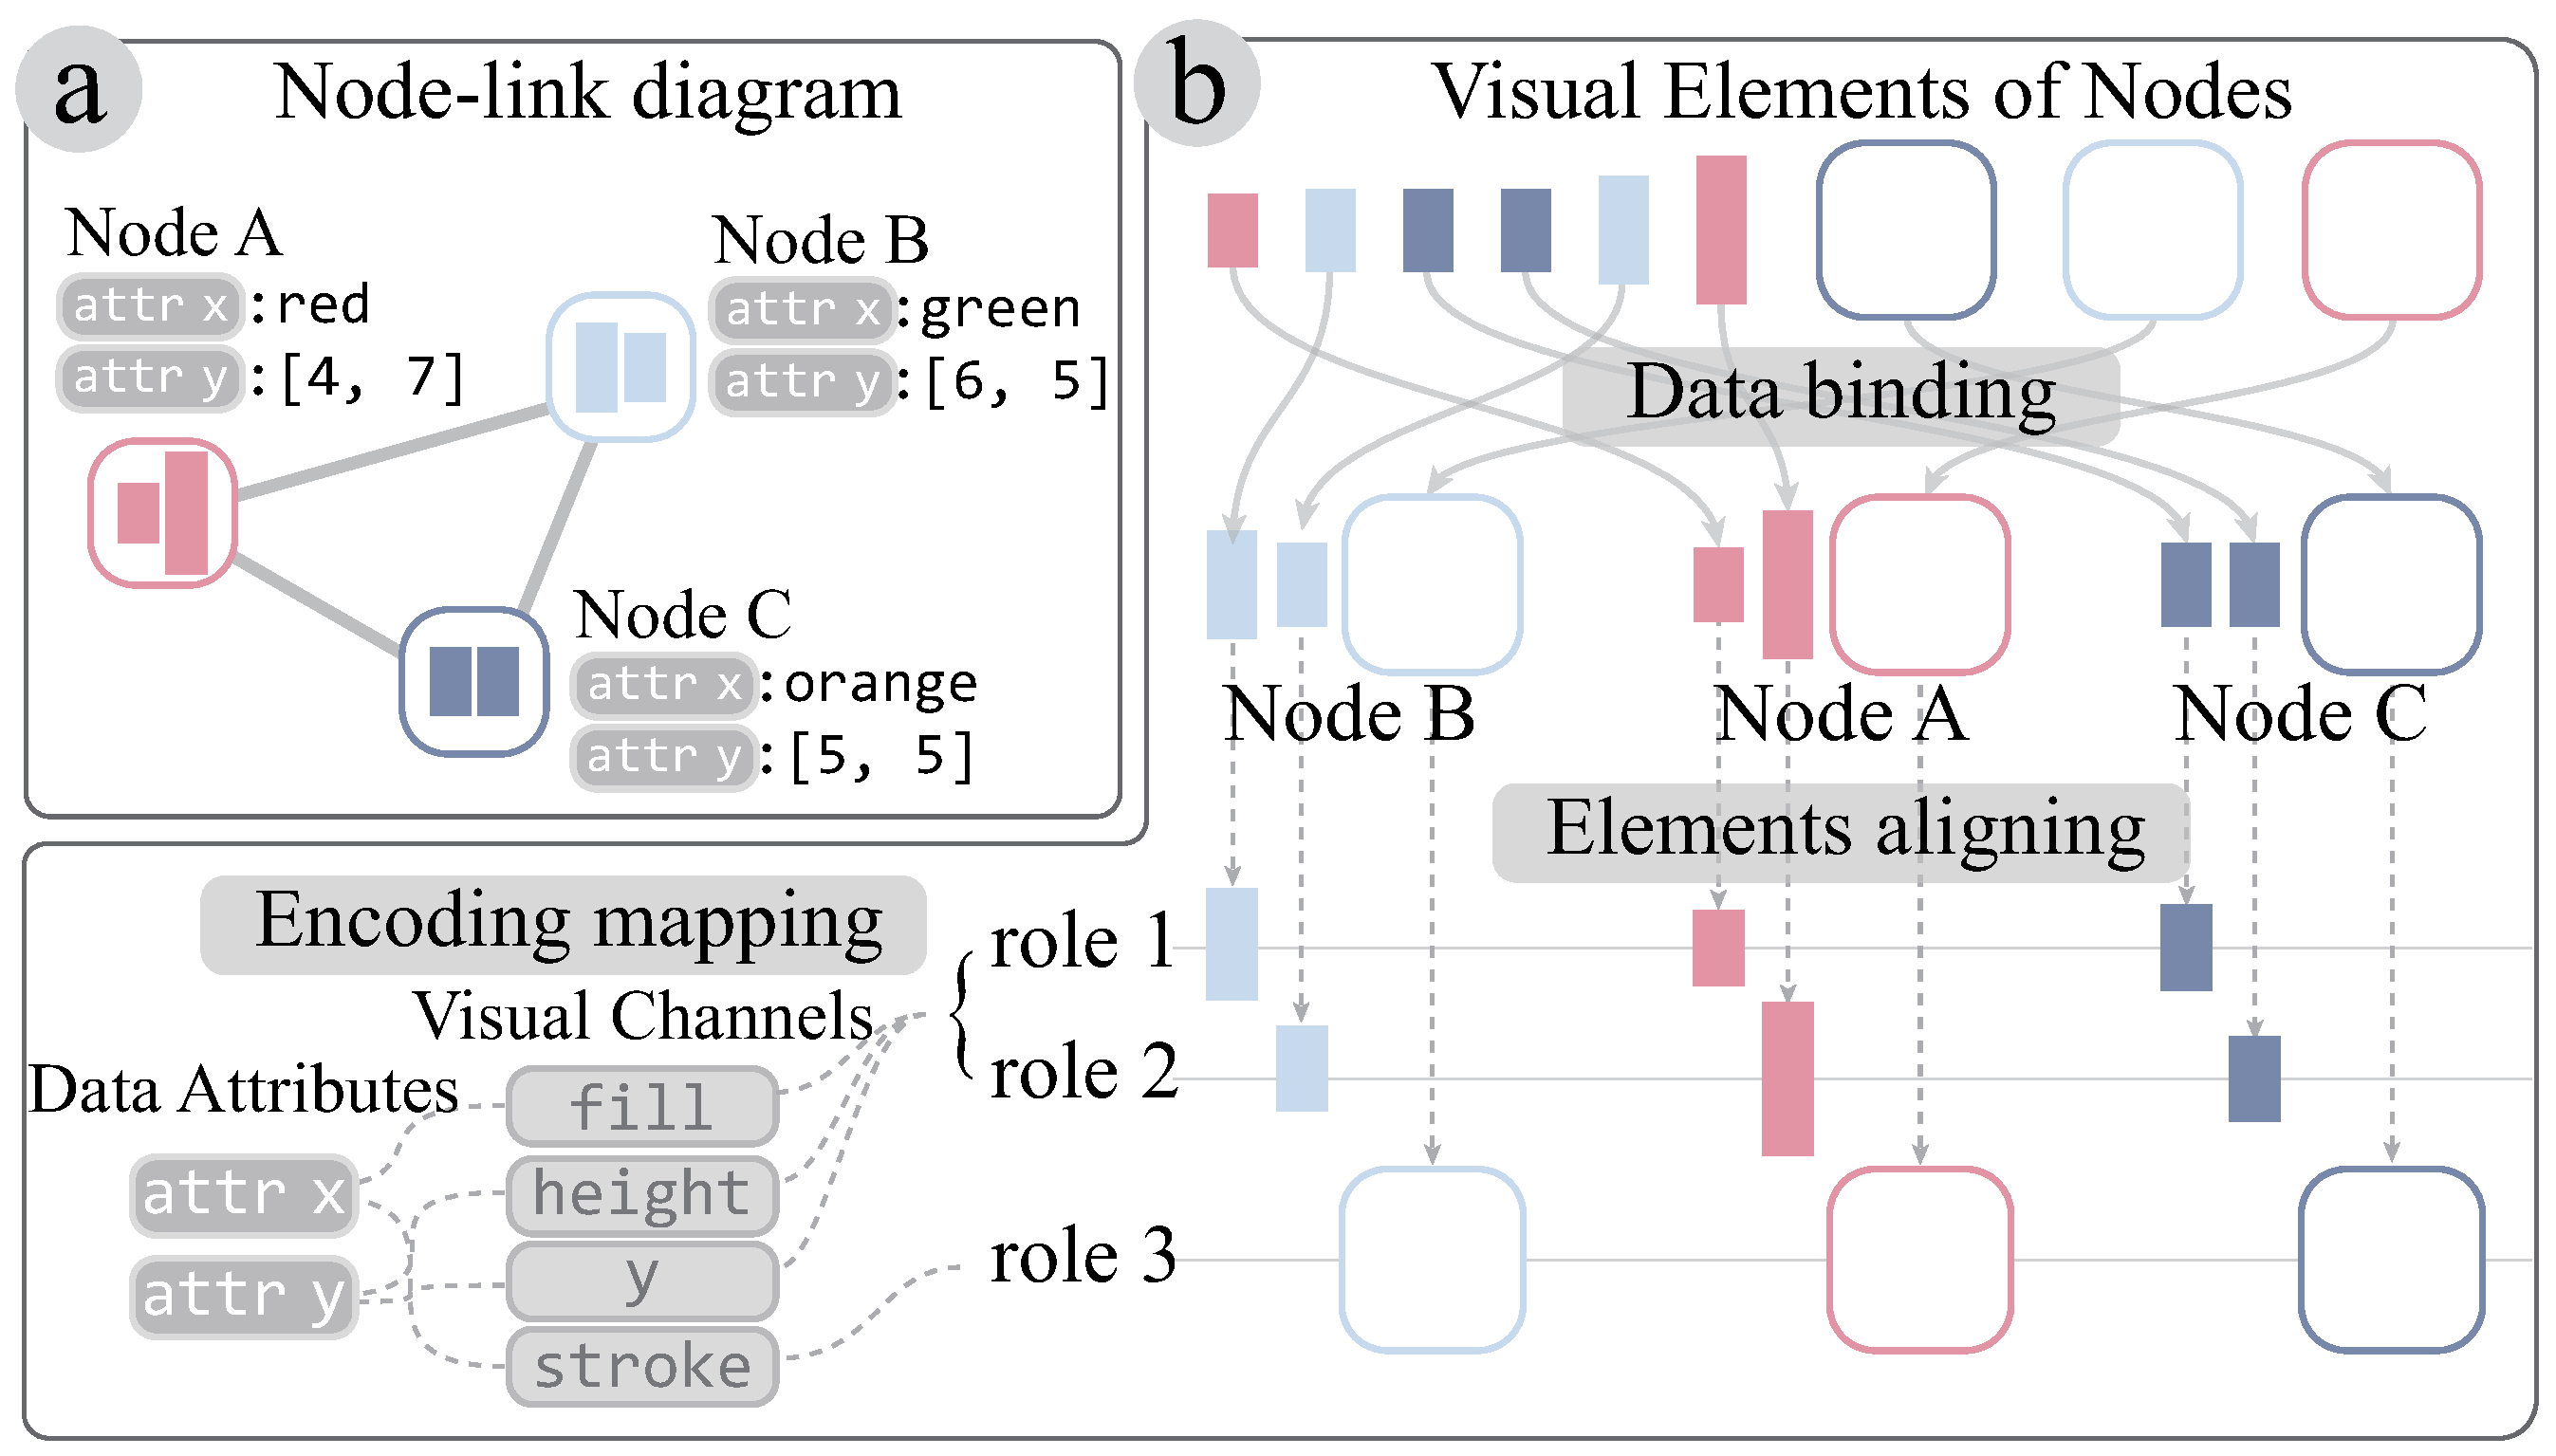
\includegraphics[width=1\columnwidth]{figures/VisualEncodings.eps}
    \setlength{\belowcaptionskip}{-10pt}
    \caption{How \ApproachName~summarizes visual encodings from a node-link diagram in the SVG format. (a) A node-link diagram consists of three nodes and three links (upper left corner). (b) Node elements are extracted and the data binding step (mapping visual elements to node entities)
    % maps them into different node entities. Then elements having the same role across different node entities are aligned into the same role class in the 2.
    the elements aligning step (aligning visual elements according to their roles),
    % Mappings among roles, visual channels, and attributes are detected by the 3.
    and the encoding mapping step (mapping data attributes to visual channels).}
    \label{fig:VisualEncodings}
\end{figure}

\begin{figure}[tp]
    \centering
    \setlength{\belowcaptionskip}{-10pt}
    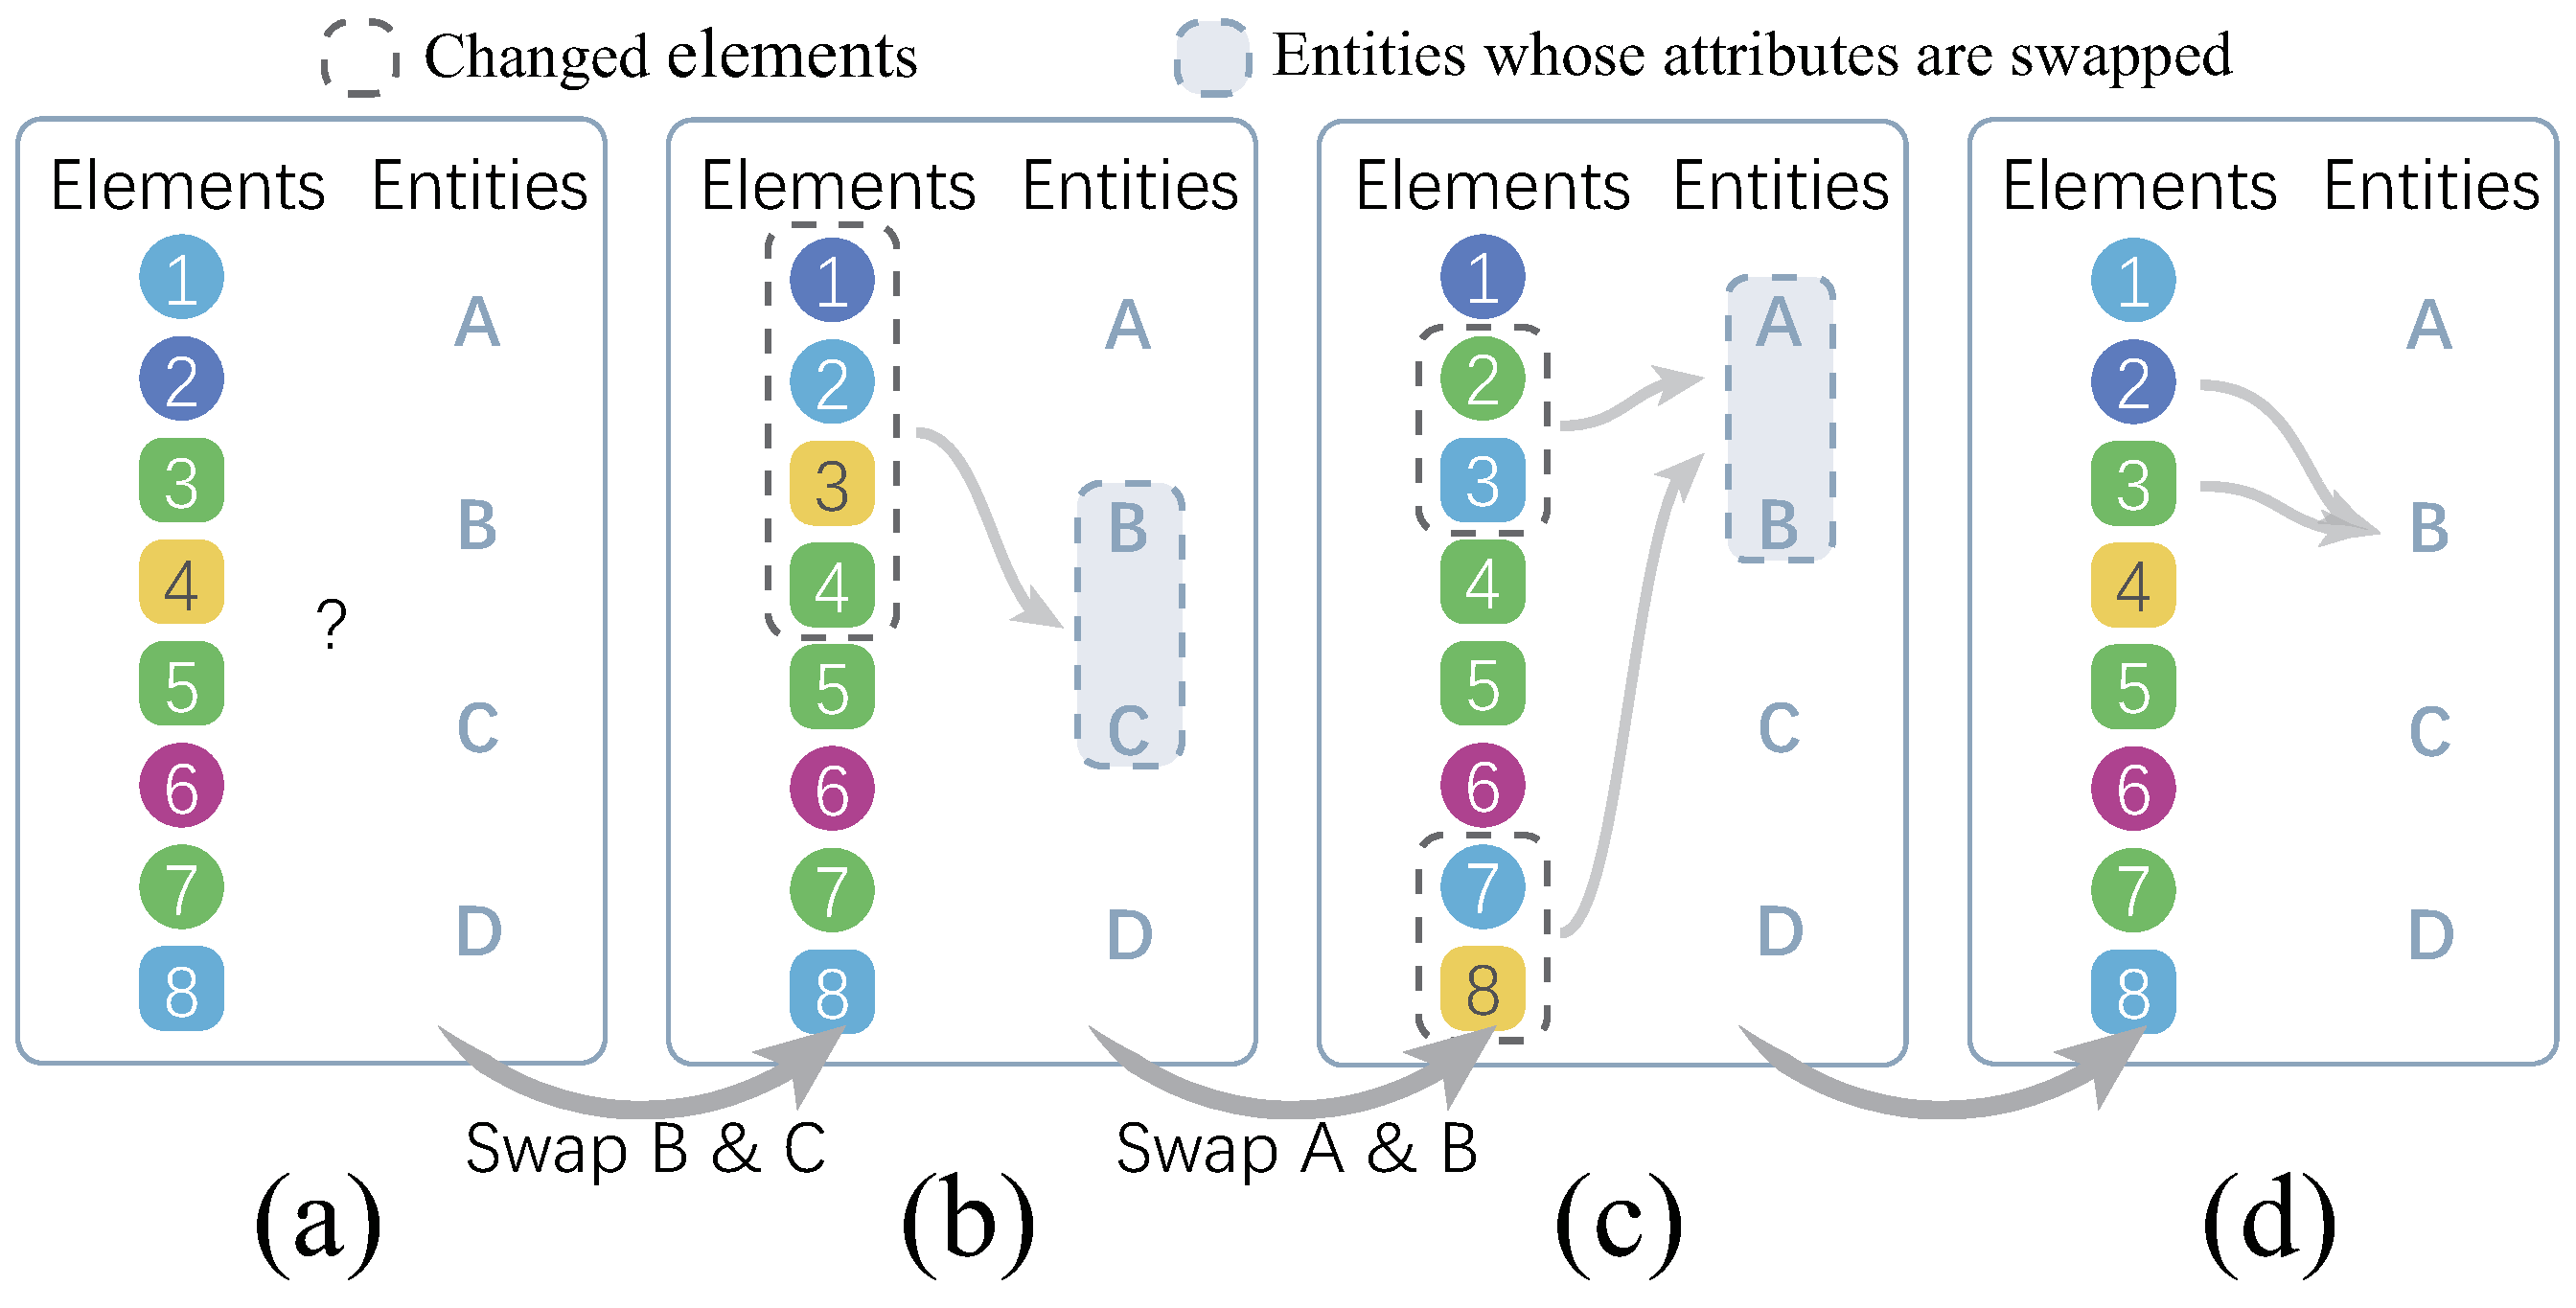
\includegraphics[width=1\columnwidth]{figures/DataBinding.eps}
    \caption{ The Data binding is achieved by swapping entities. 
    % At first, visual mappings between original visual elements and data entities are unknown. Swapping attributes of entities B and C influences the appearance of elements 1 to 4. Thus, B and C correspond to 1 to 4. Them, swapping attributes of  A and B influences 2, 3, 7, and 8. Thus, A and B correspond to these elements. Swapping B with A and C changes elements 2 and 3 twice. Thus, we map entity B to elements 2 and 3.
    }
    \label{fig:DataBinding}
    % \setlength{\abovecaptionskip}{-100pt}
    % \setlength{\belowcaptionskip}{-100pt}
\end{figure}

\begin{figure}[tp]
    \centering
    \setlength{\belowcaptionskip}{-10pt}
    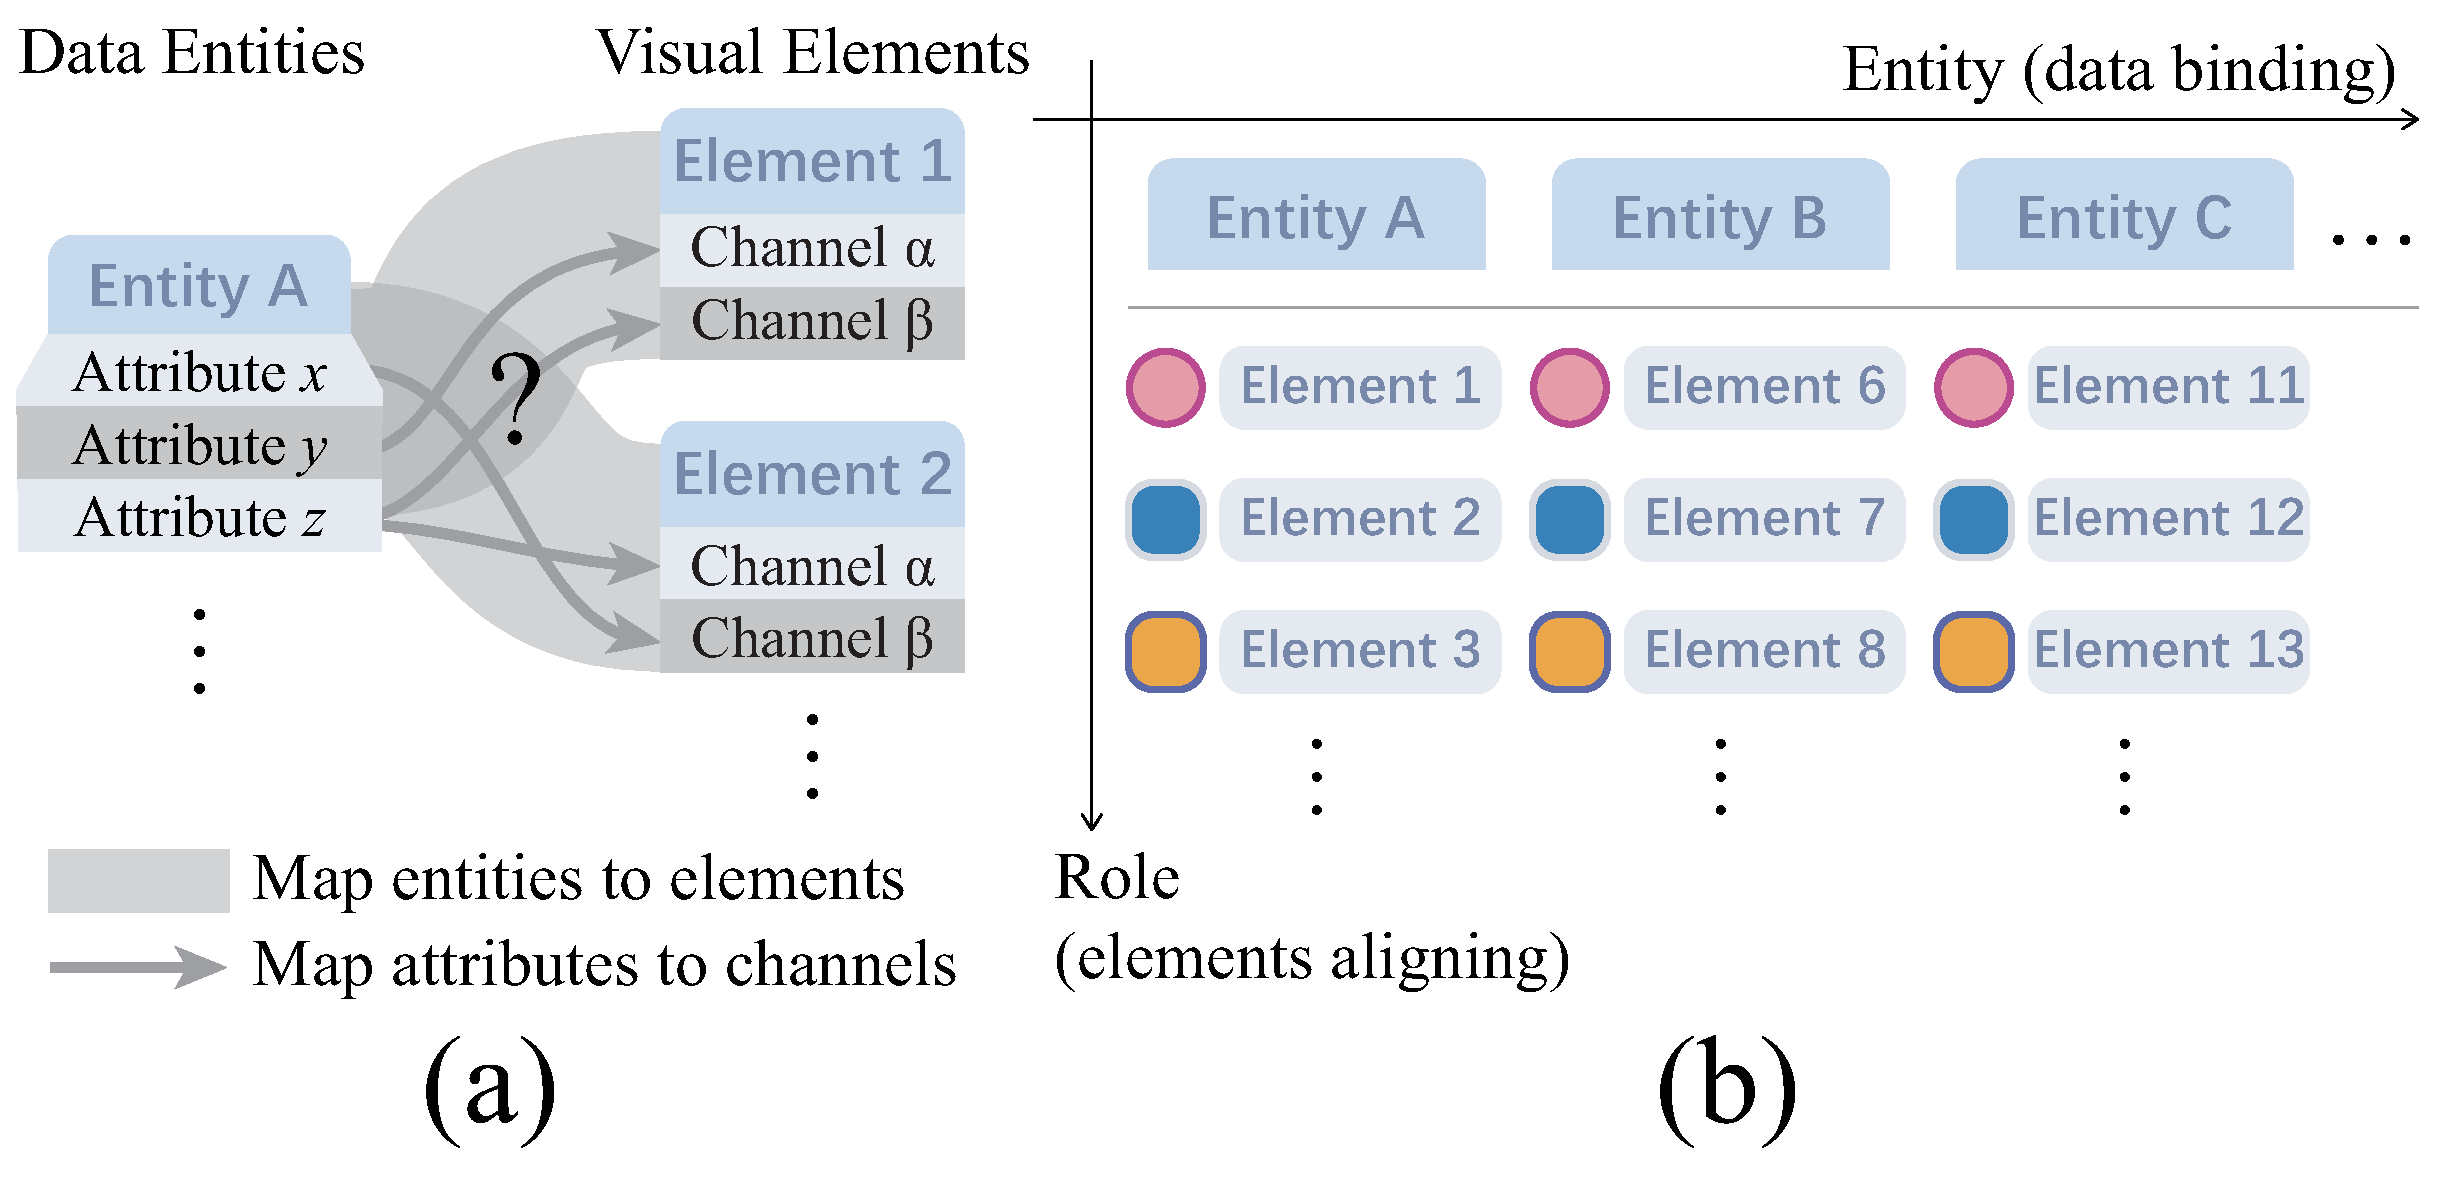
\includegraphics[width=1\columnwidth]{figures/ElementAligning.eps}
    \caption{The target of our visual encoding summarization module.
    (a) The target of the module is to find mappings among data entities, visual elements, data attributes, and visual channels. (b) To achieve the target, we utilize the data-binding step and the elements-aligning step to clarify the entity and the role of each visual element.}
    \label{fig:ElementAligning}
\end{figure}




{\bf M2.1 Data Binding.} \label{sec:databinding}
To detect mappings between \textit{data entities} and \textit{visual elements}, we modified attribute values of data entities and recorded corresponding visual element changes to construct mappings between them.
% For example, the node's \texttt{size} attribute is linearly mapped into the radius of the \texttt{<circle>} element encoding the node: 
% $radius_i = (size_i - min(size)) / (max(size) - min(size)) * radius_{max}$.
% Directly modifying $size_i$ may broaden the attribute range and changes the linear mapping defined by the attribute range.
% So that elements related to other data entities may also be changed.
% We prevent this by merely swapping attributes of the two entities rather than modifying them, so that no new data is introduced, and the distribution is preserved.
To prevent changing the distribution of attribute values, we merely swap attributes of the two entities rather than modifying them.
After swapping all two entities' attributes, visual elements that differ from the previous are regarded as two entities' corresponding elements.
For example, in Figure~\ref{fig:DataBinding} after swapping nodes B and C, elements 1 to 4 are changed.
All these changed elements correspond to nodes B and C because only B and C are modified. Then, after swapping the node B with A, elements 2 and 3 are changed twice. Thus they correspond to node B because only node B was swapped twice. Each node will be swapped with all other nodes to ensure detecting all elements belonging to it. After swapping all nodes, the entire node-to-element mapping is constructed. Thus, node entities are bound to their corresponding elements. The link-to-element mapping is constructed in the same way. Because swapping two nodes may influence their related links, node elements currently contains elements of their related links. We remove link elements from the node-to-element mappings. Two parts (\textit{entity} and \textit{element}) of the mapping relationship are solved.


{\bf M2.2 Elements Aligning.}
The data-binding step only binds visual elements into different data entities (the horizontal direction in Figure~\ref{fig:ElementAligning}b).
The roles of different elements are unknown.
The \textit{role} of an element is identified by its function in the visualization process.
We define the \textit{role} as a function that maps attributes to visual channels:
\begin{equation}
    \abovedisplayskip=5pt
    \abovedisplayshortskip=5pt
    \belowdisplayskip=5pt
    \belowdisplayshortskip=5pt
    role :=  \{attribute: value\} \mapsto \{channel: appearance\}
\end{equation}
Two elements have the same role if, given arbitrary, same inputs (all attributes of their corresponding entities) produce same outputs (all their visual channels).
For the example in Figure~\ref{fig:VisualEncodings}, 
the roles of all three left bars in node A, B, and C are the same,
because they encode same attributes with same visual channels.
% we swap all attributes of nodes A and B, node A's left rectangle before swapping will be the same as node B's left rectangle after swapping regarding all their visual channels such as x, y, fill, and height.
They are aligned to classify their roles (the vertical direction in Figure~\ref{fig:ElementAligning}b).
We determine the role of each element by swapping its data entity with others. Two elements of the same role behave the same after exchanging their data entities.
% Different elements' role identity can be determined by swapping their corresponding data entities along with the data binding step, because all attributes of one entity before swapping are the same to the counterpart of the other one after swapping.
% For instance, in Figure~\ref{fig:DataBinding}b, after swapping entity B with entity C, element 1 appears the same as element 2 before swapping in Figure~\ref{fig:DataBinding}a. Thus, elements 1 and 2 can be aligned into the same role.
We clarify the binding among visual elements, data attributes, and visual channels, which is conducive to the subsequent steps.


{\bf M2.3 Encoding mapping.}\label{sec:encodingmapping}
The previous two steps align elements according to two dimensions (the entity and the role) to clarify the relationship between data entities and visual elements.
However, correlations between visual channels and data attributes are not determined.
We detected related visual channels of an attribute by shuffling it of  all data entities and observing changes of their corresponding elements.
One correlation is defined as ``which \textit{attribute} changes which \textit{visual channel} of which \textit{element}''. We formalize it as:
\begin{equation}
    \abovedisplayskip=5pt
    \abovedisplayshortskip=5pt
    \belowdisplayskip=5pt
    \belowdisplayshortskip=5pt
    correlation := ( attribute, element, channel )
\end{equation}
We merge different correlations according to the role of elements.
Moreover, we identify the category of correlations to clarify correlations between visual channels and data attributes.
It requires the classification of attribute types and channel types.
We support numerical attributes and categorical attributes.
List attributes and dictionary attributes are separated into multiple numerical attributes or categorical attributes (e.g.,[1, 2, 3], \{"year":2021,"month":03\}).
We regard all visual channels as numerical (colors can be divided into RGB channels, which are numerical).
However, numerical data can be used as categorical data if there are only a few unique values (less than $\alpha\%$).
% For example, natural numbers are often used as categorical attributes such as labels, groups, and classes.
% Thus, for numerical data, we must compare the number of unique values and their entries to determine whether it is numerical or categorical.
% We set up a parameter $\alpha$ to make the distinction: if all values of the attribute are natural numbers and
% the number of an attribute's unique values is less than $\alpha$ a percent of the number of data entities, we regard the attribute as categorical.
We identify the type of correlation by attribute and channel types:

\noindent \textbf{Categorical correlation} -- the channel and attribute are both categorical or the channel is categorical while the attribute is numerical. 
To summarize the correlation of different channel values, we record the value range of the attribute for each channel values.
    
\noindent \textbf{Numerical correlation} -- the channel and attribute are both numerical. We compute the Pearson's Correlation Coefficient and test whether the correlation is positive, negative, or uncorrelated with the coefficient and the significance test's p-value.  The correlation is built when the absolute value of the coefficient is larger than $\theta$=.5, and the $p$-value is less than $\alpha$=.05. Both parameters can be adjusted on-demand.

We do not support the correlation type where the channel is numerical while the attribute is categorical because the former is continuous and the latter is discrete. It is counterintuitive.

\subsection{\textbf{M3}: Layout Type Identification Module}


\textbf{M3.1 Capturing the position of each node}.
Node positions are used to determine the layout type.
To capture each node's position, we compute a bounding box for elements detected in the \textbf{Data Binding} step.
It is the smallest rectangle that contains all corresponding elements.
We take its centroid as the position of the node.

\textbf{M3.2 Determining the layout type.} 
Topology-driven layouts prioritize the topology of a graph~\cite{DBLP:journals/cgf/NobreMSL19}, which means their graph geodesic distance influences the Euclidean distance between two nodes. To validate this assumption, we performed a study by using the Pearson test to check the correlation between the geodesic distance and the Euclidean distance in 15 graphs from~\cite{DBLP:journals/tvcg/ZhuCHHLZ21} layered by five topology-based layouts with default parameters (FM$^3$~\cite{hachul2004drawing}, Fruchterman-Reingold spring layout (F.R.)~\cite{DBLP:journals/spe/FruchtermanR91}, Stress Majorization (S.M.)~\cite{DBLP:conf/gd/GansnerKN04}, Pivot MDS (PMDS)~\cite{DBLP:conf/gd/BrandesP06}, and Radial Tree layout (R.T.)~\cite{DBLP:conf/infovis/Jankun-KellyM03}).
Over the total $15 \times 5 = 75$ trials, only coefficients of seven trials were less than $\theta = .5$ (see Supplementary Materials 1). And $p$-values were all zero for the five topology-based layouts in all 15 datasets.
The result indicates that in most cases, the Euclidean distance between two nodes reflects their graph geodesic distance with topology-based layouts.
Thus, it is feasible to study whether the layout is a topological layout using the Pearson correlation test.

The attribute-driven layout category consists of algorithms that map node attributes to the two dimensions ($x$ and $y$) of the Cartesian coordinate. 
We applied the Pearson correlation test to Section~\ref{sec:encodingmapping} similarly to test whether an attribute relates to the layout.

To determine the layout type, we utilize the Pearson correlation coefficient. If coefficients of the two layout types are both less than a threshold $\theta < .5$, we suggested there is no certain layout in the node-link diagram. Otherwise, the layout type with a larger coefficient is regarded as the actual layout. 
    
\begin{table*}[th]
\normalsize
\centering
\caption{The templates in the description generator. Placeholders are highlighted with a \textbf{\textit{bold italic}} font.}\label{tab:template}
\includegraphics[width=2\columnwidth]{figures/template.eps}
\vspace{-10pt}
\end{table*}

\section{Description Generator} \label{sec:generator}

\newfboxstyle{light-tight}{padding=1pt,margin=0pt,baseline-skip=false}
\fboxset{light-tight, rounded,border-style=dashed, border-radius=2pt,}%

We designed a set of templates to convert the encoded visual attributes into natural sentences (Figure~\ref{fig:workflow}b). The template is one of the most easy-to-understand ways to interpret visualization. Although many Natural Language Generation (NLG) techniques can generate more natural descriptions, the lack of training samples on node-link diagrams prevents them adapt to our scenarios. Moreover, the template is more controllable, which can be extended to different scenarios and keeps consistency.

\subsection{Description Template}

First, we present a sentence-level template by pre-setting several formats. Our template contains three parts -- 1) static texts, which bear a resemblance to the skeleton of the description and are basically consistent among different scenarios, 2) placeholders, which present the extracted information, thus are the core of our descriptions, and 3) corrections, which adapt our templates to different scenarios (e.g., replacing professional vocabulary with common words). All of our sentences which were included in the templates are listed in Table~\ref{tab:template}. For each template, we gave a sample to illustrate its input and output.

To form a logical format of these descriptions, we utilized a structure to organize them. To make the relationship among different information clear, the structures were logically organized. 

Users can obtain different levels of details in an orderly manner, where more general descriptions are shown with a higher priority.
The first part of the template is the link conditions, which help the users understand the relationship between two nodes.
The next part is the mapping between visual elements and descriptions to generate the interactive description automatically. Due to the automation characteristics, our generation approach can be promoted and adopted to lots of visualization graphs, widely benefiting millions of data news designers and stock analysts. 
The last part is the layout, because it gets the least attention from our end-users in Section~\ref{sec:pilotstudy}.
Because the visual encoding is hierarchically structured, its description generation follows a top-down scheme.
Data entities own visual elements, and visual elements have several visual channels. Some visual channels are used to encode data attributes with a certain correlation.
Thus, they are narrated hierarchically.

To reach an easy-to-understand description, professional vocabulary should be replaced. In our implementation, we replace ``tagName'' with ``shape'', ``r'' with ``radius'', ``rect'' with ``rectangle'', ``stroke\-width'' with ``thinkness'', et cetera. For colors, they are detected with their RGB values. It is obviously that describing the RGB value such as ``\#14dd39'' can not be understood by end-users (except professional designers). We build a vocabulary of 146 different color names with their values. RGB values can be replaced by uses' most similar colors in our vocabulary.


\subsection{Interactive Description}
To complete \textbf{R6}, we enable the \textit{hover-then-highlight} interaction to build mappings between descriptions and the node-link diagram. It makes descriptions more targeted.

The \textit{hover-then-highlight} is two-fold. Hovering on a description will highlight its target visual elements, and hovering on a visual element will highlight its related descriptions.
The highlight is implemented by fading irrelevant elements (Figure~\ref{fig:Movie-Actor-Jean-Pierre}b) or deepening the background color of descriptions (Figure~\ref{fig:Movie-Actor-Jean-Pierre}c).

In order to implement the interaction, we needed to clarify the visual elements related to descriptions.
In the data binding step in Section~\ref{sec:visualencodings}, we have built the relationship between data entities and visual elements. Thus, building mappings from link conditions and layout descriptions is easily achieved. Layout type descriptions highlight node visual elements, while links conditions emphasize link elements. For descriptions of visual encodings, elements to highlight are selected by a filtering mechanism. For instance, in Figure~\ref{fig:Movie-Actor-Jean-Pierre}c, the hovered description tells a color encoding to highlight only the elements that coincide to the description (steelblue nodes) (Figure~\ref{fig:Movie-Actor-Jean-Pierre}b).
 

In addition, to support the hierarchy, we implement a \textbf{collapse} interaction to clarify the ownership of different descriptions (Figure~\ref{fig:Movie-Actor-Jean-Pierre}c). Users can click 
\includegraphics[height=0.8\baselineskip]{figures/collapse-symbol-1.eps} and 
\includegraphics[height=0.8\baselineskip]{figures/collapse-symbol-2.eps} symbols at the beginning of the texts to toggle more detailed descriptions.



\begin{figure}[tp]
    \centering
    \setlength{\belowcaptionskip}{-10pt}
    \includegraphics[width=1\columnwidth]{figures/Movie-Actor-Jean-Pierre.eps}
    \caption{Case 1: Usage Scenario. (a) is the node-link diagram created with the Movie-J.P.M. graph (14 nodes and 25 links). (b) When the user hovers on a node, its related descriptions will be highlighted in (c).}
    \label{fig:Movie-Actor-Jean-Pierre}
\end{figure}
    \section{Case Studies} \label{sec:casestudy}

To show the usage scenarios and usability of our~\ApproachName, we designed and conducted three case studies with different link conditions, layout types, and flexible visual encodings.
Based on the IMDb dataset~\cite{IMDb-extensive-dataset} as others did~\cite{DBLP:conf/ieeevast/BigelowNML19, DBLP:journals/ivs/LiuNS14, DBLP:journals/tkde/HerschelNST12}, we generated three graphs and designed their corresponding node-link diagrams. Table~\ref{tab:case-graph} shows their detailed information.

\begin{table*}[t]
\normalsize
\centering
\caption{The proposed graphs used in case studies. }\label{tab:case-graph}
\includegraphics[width=2\columnwidth]{figures/case-graphs.eps}
\vspace{-10pt}
\end{table*}


\subsection{Case 1: Usage Scenario}
This case shows a basic usage scenario. 
Three kinds of information following E1-3 are generated: link conditions, visual encodings, and the layout type.

\noindent \textbf{Link Conditions}.~\ApproachName~recognizes the link condition ($type$=C2, $attribute$=actors, $value$=arbitrary) and thus generates a description in Figure~\ref{fig:Movie-Actor-Jean-Pierre}b line 1.

\noindent \textbf{Visual Encodings}. Nodes are visualized with two different shapes: circles and rectangles.
To distinguish the encoding scheme in different shapes,~\ApproachName~describes them separately.
First, the ``country'' attribute encoded on the shape is narrated (Figure~\ref{fig:Movie-Actor-Jean-Pierre}c, line 3, 4, and 6).
Details of the two shapes are described in line 5, and 7-8.

\noindent \textbf{Layout Type}.
The layout is attribute-based.~\ApproachName~detects the encoding attributes on two coordinates (year and duration) and generates descriptions in Figure~\ref{fig:Movie-Actor-Jean-Pierre}c, line 17-21.

\noindent \textbf{The Hover-then-highlight Interaction}.
The interaction enables users to obtain the targets of descriptions. For instance, hovering line 11 in Figure~\ref{fig:Movie-Actor-Jean-Pierre}c highlights the corresponding elements in Figure~\ref{fig:Movie-Actor-Jean-Pierre}b. So that users can clarify that the description target is the steelblue nodes.


\begin{figure}[tp]
    \centering
    \includegraphics[width=1\columnwidth]{figures/Movie-Year-Nolan.eps}
    \setlength{\abovecaptionskip}{-5pt}
    \setlength{\belowcaptionskip}{-10pt}
    \caption{Case 2: Glyph Design on Link. (a) is the node-link diagram based on the Movie-C.N. graph (11 nodes and 16 links). (b) Several nodes are highlighted when the user hovers on one of their related descriptions in (c).}\label{fig:Movie-Year-Nolan}
\end{figure}

\subsection{Case 2: Glyph Design on Links}
Case 2 (Figure~\ref{fig:Movie-Year-Nolan}) is designed to demonstrate~\ApproachName's ability of dealing with different link conditions and complex visual encodings on links. The design of the node-link diagram follows~\cite{DBLP:conf/iv/SchoffelSE16}. Links are encoded with several bars to display link attributes. It is hard to distinguish the roles of different visual elements in encoding attributes. Our~\ApproachName~gives an amazing performance in analyzing of such visual design.

\noindent \textbf{Link Conditions}. 
First,~\ApproachName~detects the link condition of the node-link diagram ($type$=C3, $attribute$=year, $value$=5) and describes it in Figure~\ref{fig:Movie-Year-Nolan}c, line 1.

\noindent \textbf{Visual Encodings}. 
Although each link has nine visual elements, only four rectangles encode attributes.
Thus, our descriptions only narrate the four rectangles with attributes encoded in Figure~\ref{fig:Movie-Year-Nolan}c, line 7-18.
End-users can focus on the informative visual elements and ignore the others without visual encodings.

\noindent \textbf{Layout Type}.~\ApproachName~detects the force-directed layout. We directly utilize the template to describe it (Figure~\ref{fig:Movie-Year-Nolan}c, line 19).

\noindent \textbf{The Hover-then-highlight Interaction}.
When hovering over certain visual elements, their correlated descriptions will be highlighted with a gray background. For example, in Figure~\ref{fig:Movie-Year-Nolan}(b and c), hovering the red rectangular on a link toggles descriptions in line 1 and 6-9.

\subsection{Case 3: Bar Charts Nested on Nodes}
In this case, we demonstrate~\ApproachName's ability to explain a complex node-link diagram with nested charts on nodes. It follows the design of~\cite{DBLP:journals/bmcbi/JunkerKS06}, where each node nests a chart (Figure~\ref{fig:teaser}). This case is used to illustrate visual encodings, and thus we do not discuss other descriptions here.

\noindent \textbf{Visual Encodings}
In each node, five <rect> (rectangle) elements are composed together to encode the actors' activeness, namely the number of movies they acted in each year.
To help end-users understand such an encoding scheme, our~\ApproachName~generates fine-grained descriptions to narrate each rectangle's encoding scheme (Figure~\ref{fig:teaser}d visual encodings).
One benefit of such descriptions is that users can understand the information encoded on each rectangle (numbers of movies the actor acted in from 2016 to 2020) rather than only an abstract description such as \textit{``encoding the actor's activeness''}.

    \section{User Study}

\begin{figure}[tp]
    \centering
    \setlength{\belowcaptionskip}{-25pt}
    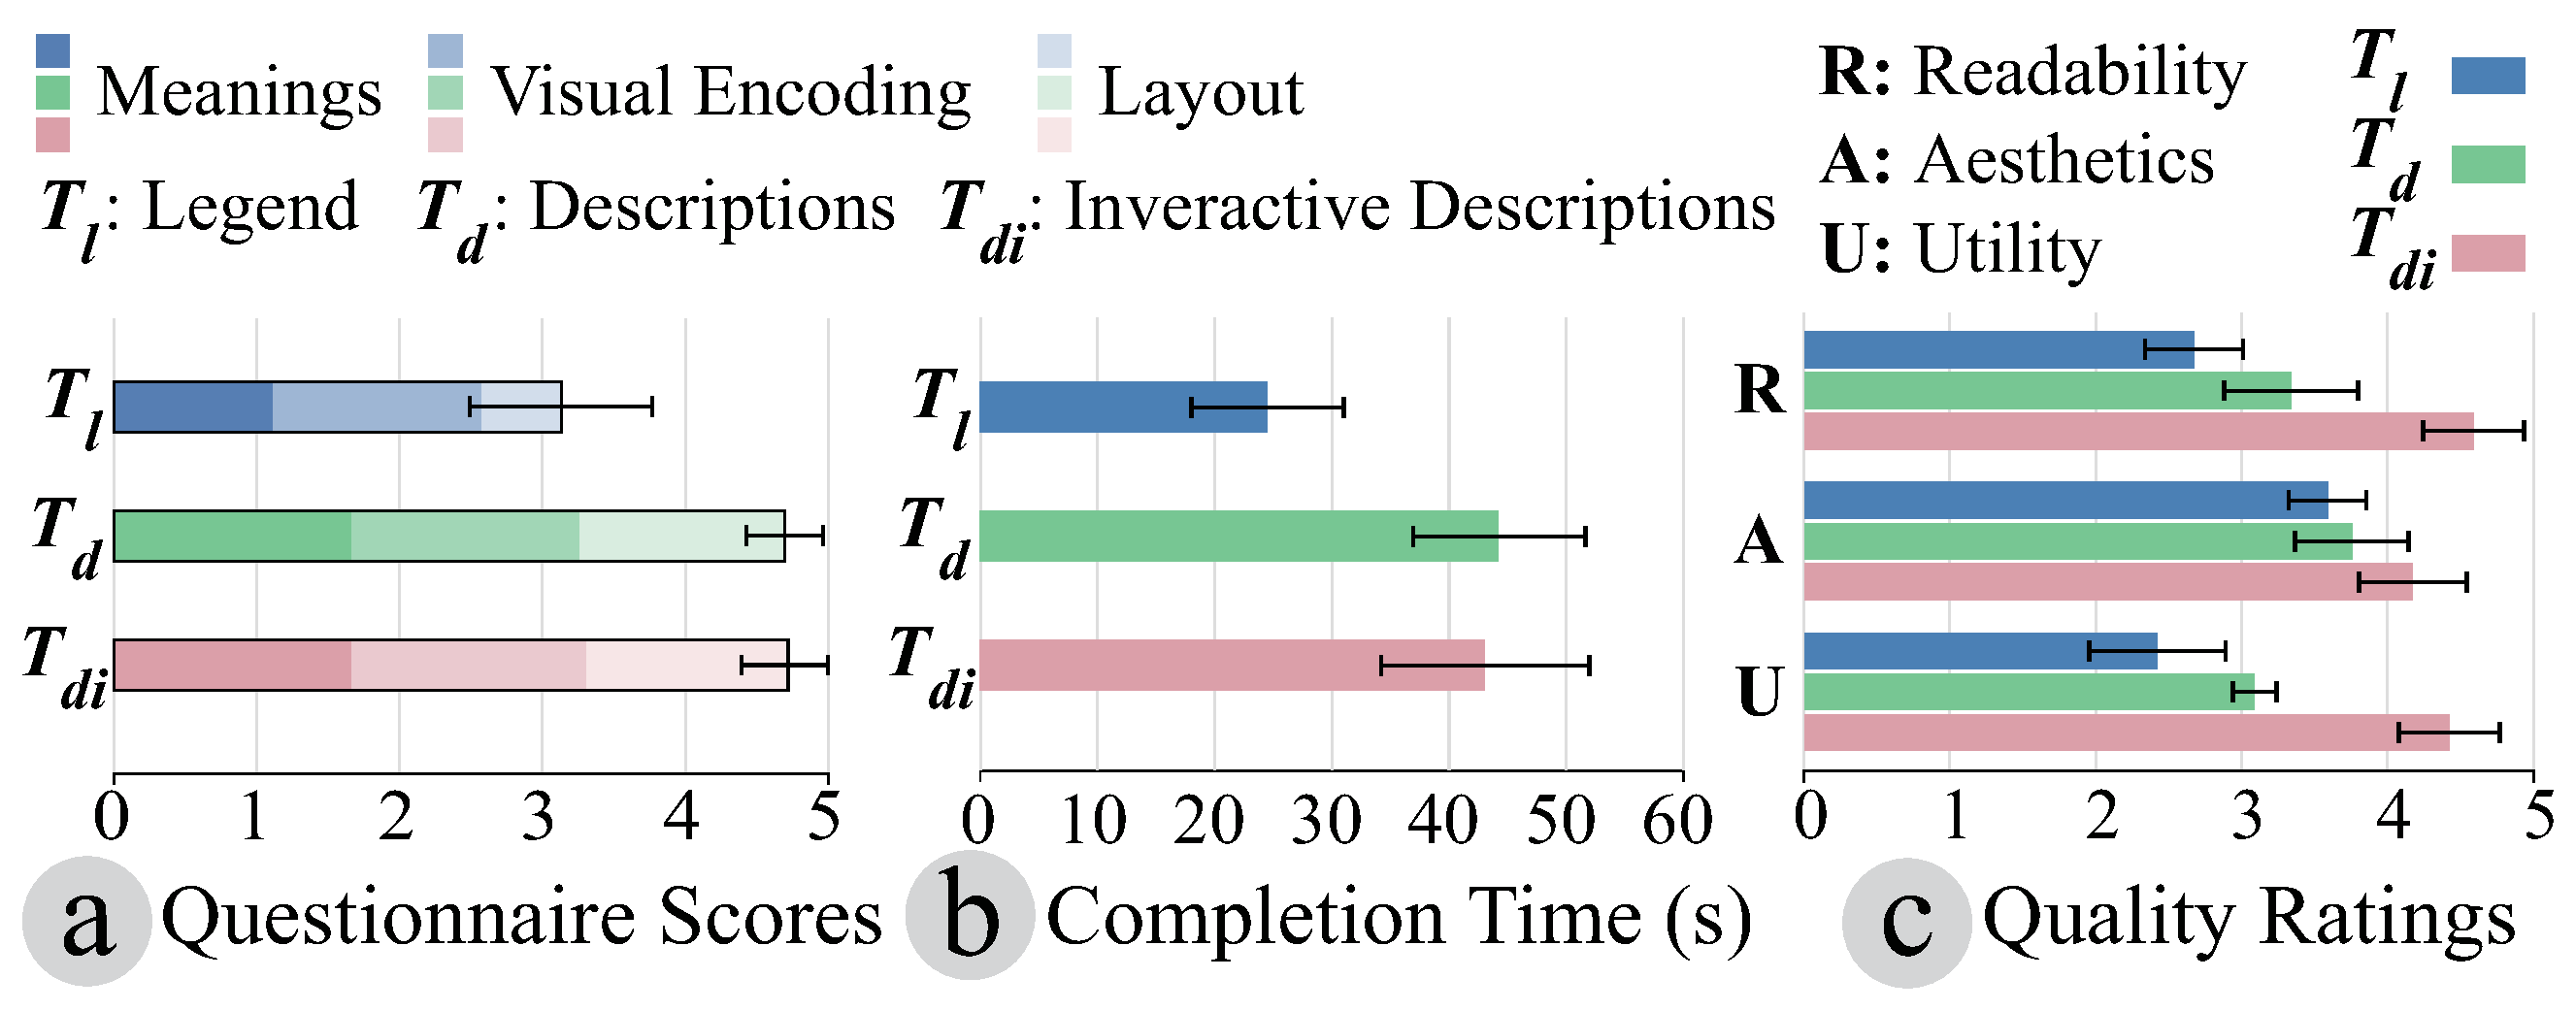
\includegraphics[width=1\columnwidth]{figures/UserStudy.eps}
    \caption{The result of our user study with the mean values of $95\%$ confidence intervals. (a) The questionnaire score distributions of three techniques, (b) the average completion time distributions of three techniques, and (c) the distribution of ratings of different metrics of our interactive descriptions. }
    \label{fig:UserStudy}
\end{figure}


We conducted a qualitative user study to assess the effectiveness of~\ApproachName. The study aimed to evaluate whether our approach can enhance the comprehensibility of node-link diagrams. This study chooses one of the most classic scheme -- the legend, as our baseline. We evaluated our approach's effect on comprehensibility enhancement by comparing the effect of the legend, our generated descriptions, and descriptions without interactions.


\textbf{Participants.}
We recruited 12 participants in the study (P1-P12; 4 males; aged: 22-26 ($\mu$=23.58, $\sigma$=1.32)). All participants are students or researchers from the Computer Science department, three of them majored in Visualization with professional experience in analyzing node-like diagrams, and the others have the basic visualization knowledge by taking the relevant courses. The scale of expert participants is consistent with similar graph visualization research~\cite{DBLP:journals/tvcg/BehrischSP20, DBLP:journals/tvcg/YoghourdjianDKM18}. Each participant received a gift card worth \$15 at the beginning, independent of their performance.


\textbf{Task. }
We chose the three node-link diagrams used in Section~\ref{sec:casestudy} as our test material. We prepared three types of descriptions: $T_l$ is the legend, which serves as the control group, $T_d$ is our descriptions without interaction, and $T_{di}$ is our interactive descriptions. For the legend, there is no standard design to convey information about the layout type. Our legends design only displays the layout type with text (``topology'') and axes (attributes). For each diagram, there will be 
several detailed descriptions samples (ten in case 1, eight in case 2, and eight in case 3) with different types of information (link conditions, visual encodings, and layout type).  To sum up, a complete task contains: 3 \emph{descriptions conditions} $\times (10+8+8)$ \emph{samples} = 78 trials. 

\textbf{Procedure. }
The study began with an introduction (three minutes) of the study purpose, study materials and the study tasks. During the practice phase (five minutes), participants were equipped with a mouse to explore node-link diagrams, legends, and descriptions freely.

After the training, participants started the formal tasks, which lasted for around one hour. We recorded the exploration time and successfulness of each trial. Each trial ended with a post-study questionnaire (one minute) to evaluate the understanding degree of users, which reflects the comprehensibility of our approaches. The questions for the three diagrams are consistent with the three parts of information summarized in Section~\ref{sec:pilotstudy}. 
The total score of one participant was scaled to a five-point score.

After each task, participants were asked to rate four five-point Likert scale questionnaires regarding readability, aesthetics, and utility. Besides, they were encouraged to give suggestions for our techniques.

\subsection{Results, Findings and Lesson Learned}
We consider that the study assessed the system qualitatively rather than quantitatively due to the small sample size. 


\textbf{Comprehensibility}.
The higher the score, the better comprehensibility of node-link diagrams. Overall, the results of $T_d$ ($\mu$=4.72, $\sigma$=.94), $T_{di}$ ($\mu$=4.70, $\sigma$=.79)) and $T_l$ ($\mu$=3.13, $\sigma$=1.86) are shown in Figure~\ref{fig:UserStudy}a. For non-parametric statistical significance test results, the Friedman test suggests significance among three techniques ($p<.05$), and the Wilcoxon Signed-Rank test suggests $T_l$ gets lower scores than both $T_d$ and $T_{di}$ ($p<.05$). No significance is suggested between $T_d$ and $T_{di}$ ($p=.72$). 
We repeated the two tests on the scores of different description types (link conditions, visual encodings, and layout type), and found that $T_d$ and $T_{di}$ were significantly better than $T_l$ while no significance was detected between $T_d$ and $T_{di}$.
The results reported that our two techniques enhanced the comprehensibility of node-link diagrams compared with the legend.
Most of the participants commended our descriptions: \textit{``I do not need to speculate information when viewing descriptions. They are comprehensive and precise.''} 

\begin{itemize}[noitemsep,topsep=0pt,parsep=0pt,partopsep=0pt, leftmargin=20pt]
    \item {\bf Finding 1}: 
    The comprehensibility improvement made by our descriptions mainly comes from the completeness of needed information. The hover-then-highlight interaction helps little to the comprehensibility.
    \item {\bf Lesson Learned 1}: 
    To augment comprehensibility, we can explore other interaction methods and develop more comprehensive descriptions.
\end{itemize}

{\bf Efficiency.} Users reported that the relatively high information granularity of our descriptions makes them spend more time on exploration and relevant information selection. And the analysis on completing time supports their report. 
By employing the two non-parametric statistical significance tests, we find the time of using $T_d$ ($\mu$=44.25, $\sigma$=11.01) and $T_{di}$ ($\mu$=43.10, $\sigma$=13.40) is significantly higher ($p$<.05) than $T_l$ ($\mu$=24.51, $\sigma$=9.81).
We also find there is no significant difference between $T_d$ and $T_{di}$ ($p=.58$). Our interaction has little impact on the exploration time of the task.

\begin{itemize}[noitemsep,topsep=0pt,parsep=0pt,partopsep=0pt, leftmargin=20pt]
    \item {\bf Finding 2}: Exhaustive description costs people more time to explore and select information.
    \item {\bf Lesson Learned 2}: We need to balance the comprehensiveness and conciseness of information. We can highlight some partial information on the descriptions according to usage scenarios and user preferences.
\end{itemize}


\textbf{Utility}.
We found that our participants rated the utility of $T_{di}$ ($\mu$=4.42, $\sigma$=.67) significantly higher than $T_d$ ($\mu$=3.08, $\sigma$=.29), and the utility of $T_d$ is also significantly higher ($p$<.05) than $T_l$ ($\mu$=2.42, $\sigma$=.90).
It means our participants prefer interactive descriptions.
P10 said the interaction attracted his interest to read the description.
P3 mentioned that the spatial relationship between descriptions and the node-link diagram affected his information searching and mapping.
Two participants (P5 and P11) suggested generating tooltips to show the information of each data entity.

\begin{itemize}[noitemsep,topsep=0pt,parsep=0pt,partopsep=0pt, leftmargin=20pt]
    \item {\bf Finding 3}: The distance between descriptions to visualization affects the utility.
    \item {\bf Lesson Learned 3}: We need to consider the spatial relationship between visualization and descriptions. And the tooltip might be an alternative to the current hover-then-highlight interaction.
\end{itemize}

\textbf{Aesthetics}.
The Friedman significance test suggested there is no significance among our descriptions and the legend ($p$=.08).
P1 commented that \textit{``Text colors of descriptions are a little complex.''} She suggested reducing the design complexity by using fewer fonts and colors to highlight essential information.

\begin{itemize}[noitemsep,topsep=0pt,parsep=0pt,partopsep=0pt, leftmargin=20pt]
    \item {\bf Finding 4}: Over-considering the information does not improve readability, but also increases cognitive load for users.
    \item {\bf Lesson Learned 4}: we should rank the importance of different information, and only highlight the most important information.
\end{itemize}

\textbf{Readability}.
Two significance tests suggested that $T_{di}$ ($\mu$=4.50, $\sigma$=.80) is more readable than $T_d$ ($\mu$=3.33, $\sigma$=.89) and $T_l$ ($\mu$=2.67, $\sigma$=.65). And $T_d$ makes no difference to $T_l$.
Although our interaction helps to improve the comprehensibility a bit, it improves the readability of our descriptions.
Most of our participants praised our interaction design, such as \textit{``The interaction locates the target visual elements for me to track and solve questions.''} 
P10, who gave a low score for the readability, commented that descriptions of visual encodings were too trivial for him to find the required information. 
He suggested replacing trivial and repetitive text with symbols, such as icons and arrows.
% Another participant suggested us to generate descriptions with multilingual versions. It can help non-native English users to understand node-link diagrams.
 

\begin{itemize}[noitemsep,topsep=0pt,parsep=0pt,partopsep=0pt, leftmargin=20pt]
    \item {\bf Finding 5}: Trivial and repetitive templates affect the readability of descriptions.
    \item {\bf Lesson Learned 5}: We should explore more organizing forms of descriptions. And replacing repetitive texts with icons such as arrows and emojis may improve the readability.
\end{itemize}


    \section{Discussion}

\noindent {\bf Significance--using textual descriptions.}
\ApproachName~makes it possible for end-users to understand complicated node-link diagrams. Unlike traditional design only express information with simple representations, such as legends, our approach can provide more detailed and concise descriptions. We also found that interactive descriptions can ease users' understating compared with static ones. Moreover, it indicates opportunities for future visualization design and analytics, benefiting not only normal users but also experts. The generated description can help developers debug, modify and re-generate their node-link diagrams quickly, and help designers optimize visual representation logically.


\noindent {\bf Generalizability--extending to other visualization and scenarios.}
\ApproachName~can be applied to other visualization types because different types of visualization are somewhat related and similar. For instance, scatterplots can be viewed as graphs without any link. Thus, our approach can summarize their visual encodings. Moreover, the overall idea of deconstruction visualization can be extended to more scenarios. For instance, we can explain the scatterplot-based dimension reduction algorithm depicting the mainly correlated feature.

\noindent {\bf Comprehensibility--augmenting the design of descriptions}. 
Although our interactive description is practical, some users suggest exploring more information representation and interaction approaches, such as tooltip. One possible optimization is to balance the comprehensiveness and conciseness of the description. We propose three methods to reach this goal. First, Integrate different types of information and thus reduce the repetitive descriptions. Second, hybrid icons and emojis into descriptions to make them more pleasant and concise. Third, apply the shortest distance principle to the placement of the description. In this case, relevant descriptions can be placed near the target visual element, helping users understand the mapping.


\noindent {\bf Scalability-generating large-scale descriptions}.
\ApproachName~has three modules. We analyze the time's complexity of each, respectively. Link conditions searching modules (M1) must traverse all pairs of nodes to find potential conditions. Its time complexity is $O(N^2)$, where $N$ is the number of nodes.
Visual encodings summarizing (M2) need to swap all pairs of nodes and links, and then traverse and compare all elements to obtain their differences.
The number of elements is linear in the number of data entities, so time complexity is $O(N^3 + M^3)$, where $M$ is the number of links.
Detecting visual mappings between attributes and visual channels requires shuffling values of attributes and observing changes in visual channels.
Thus its time complexity is $O(N \times (K_{An} + K_{Cn}) + M \times  (K_{Al} + K_{Cl}))$, where $K_{An}$ and $K_{Al}$ are numbers of attributes on nodes and links, and $K_{Cn}$ and $K_{Cl}$ are numbers of visual channels on nodes and links.
Layout type Identifying M3 requires the computation of two distance matrices.
Finding the shortest paths of all node pairs is $O(N^3)$.
The most time-consuming part is interpreting visual encodings, because a new SVG element must be generated for each swap, and visual channels for each element must be computed.
By implementing our algorithm on the server-side,
the generation of SVG elements and the computation of visual channels can be accelerated.
Besides, for larger-scale node-link diagrams, sampling techniques can be employed for acceleration.

\noindent {\bf Limitations and future work.}
There are several limitations for~\ApproachName.
First, our approach builds upon one assumption that the diagram is consistent. If different parts of the graph are handled differently, for example, nodes are encoded by different encoding schemes,~\ApproachName~cannot extract all these features according to our expectations. 
However, these cases are infrequent and can be mitigated by adding classification strategies to distinguish different parts with disparate schemes.
Second, our approach is designed for web-based visualization. The web environment enables us to ignore the collection of data and visualization programs because network traffic investigation tools can easily capture them. And the SVG-based node-link diagrams make~\ApproachName~possible to deconstruct the visualization results.
Collecting data and programs and deconstructing non-SVG-based visualization are not considered yet.
Third, the types of link conditions and layouts are limited. We focus on specific types according to some existing research currently~\cite{DBLP:journals/tvcg/SrinivasanPEB18, DBLP:conf/ieeevast/BigelowNML19, DBLP:journals/cgf/NobreMSL19}, but we can explore more kinds of link conditions and layout types in the future.
    \section{Conclusion}
In this paper, we have introduced an automatic approach,~\ApproachName, to extract and express information with descriptions for node-link diagrams.
To understand how node-link diagrams are constructed and what should be explained, we have conducted a pilot study with three graph experts and 12 participants to explore the design of our approach.
We formulated two categories of requirements for~\ApproachName~including four extraction requirements and two expression requirements.
Accordingly, we separate the design of~\ApproachName~into two parts: 1) Three modules search link conditions, summarize visual encodings, and identify layout types. It follows the idea of deconstructing node-link diagrams by inferring the information from visualization results.
2) An description generator organizes template-based descriptions following a pre-set scheme. It constructs a linkage between the visualization and descriptions to enable interactions.
Three case studies and the results from an in-lab study show that~\ApproachName~can effectively express the node-link diagram and help end-users get clear understanding of the visualization.

\fi

%% if specified like this the section will be committed in review mode
\acknowledgments{
}

\bibliographystyle{abbrv}
%%use following if all content of bibtex file should be shown
\nocite{}
\bibliography{template}
\end{CJK} %! FOR CHINESE
\end{document}

